\documentclass[lualatex,aspectratio=169]{beamer}
\usepackage[T1]{fontenc}
\usepackage{luatexja}
\usepackage{luatexja-ruby}
\usepackage[deluxe]{luatexja-preset} 
\usepackage{amsmath}
\usepackage{tikz}
\usepackage{caption}
\usepackage{listings}
\lstset{
  basicstyle=\footnotesize\ttfamily,
  keywordstyle=\color{blue},
  language=[LaTeX]TeX,
  breaklines=true,
  showstringspaces=false,
}
\captionsetup[figure]{labelformat=empty}
\setmainjfont{Hiragino Kaku Gothic ProN}

\usetheme[progressbar=none]{metropolis}

\usepackage{pifont}
\newcommand{\cmark}{\ding{51}}%
\newcommand{\xmark}{\ding{55}}%

\usepackage{xcolor}
\definecolor{hf-orange}{HTML}{FFA700}
\definecolor{hf-orange-dark}{HTML}{FF882B}
\definecolor{hf-blue}{HTML}{4884DA}
\definecolor{hf-blue-dark}{HTML}{4D6BD5}
\definecolor{hf-orange-gradient-left}{HTML}{FF882B}
\definecolor{hf-orange-gradient-right}{HTML}{FFE721}
\definecolor{hf-blue-gradient-left}{HTML}{48D2E6}
\definecolor{hf-blue-gradient-right}{HTML}{4D6BD5}
\definecolor{white}{HTML}{FFFFFF}

\setbeamertemplate{footline}{%
  \begin{tikzpicture}[remember picture, overlay]
    % left half of the bar
    \shade[left color=hf-orange-gradient-left, right color=hf-orange-gradient-right]
      (current page.south west) rectangle ([yshift=0.5mm]current page.south);

    % right half of the bar
    \shade[left color=hf-blue-gradient-left, right color=hf-blue-gradient-right]
      (current page.south) rectangle ([yshift=0.5mm]current page.south east);

    % slide number
    \node[
      anchor=east,
      xshift=-5mm,
      yshift=5mm,
      font=\sffamily\color{mDarkTeal}
    ]
    at (current page.south east)
    {\insertframenumber};
  \end{tikzpicture}%
}

\setbeamertemplate{title separator}{
  
\begin{tikzpicture}
    % Left half of the bar
    \shade[left color=hf-orange-gradient-left, right color=hf-orange-gradient-right]
      (0,0) rectangle (0.5\textwidth, 0.25mm);
    % Right half of the bar
    \shade[left color=hf-blue-gradient-left, right color=hf-blue-gradient-right]
      (0.5\textwidth,0) rectangle (\textwidth, 0.25mm);
  \end{tikzpicture}
  \vskip1em % Adds a little vertical space after the separator
}

\setbeamertemplate{section page}{
  \begin{center}
    \usebeamerfont{section title}
    \usebeamercolor[fg]{section title}
    \insertsection
    \par % Creates a new paragraph for spacing
    
\begin{tikzpicture}
      % Left half of the bar
      \shade[left color=hf-orange-gradient-left, right color=hf-orange-gradient-right]
        (0,0) rectangle (0.5\textwidth, 0.25mm);
      % Right half of the bar
      \shade[left color=hf-blue-gradient-left, right color=hf-blue-gradient-right]
        (0.5\textwidth,0) rectangle (\textwidth, 0.25mm);
    \end{tikzpicture}
  \end{center}
}

\setbeamercolor{frametitle}{fg=mDarkTeal, bg=black!2}
\setbeamertemplate{frametitle}{
  \nointerlineskip%
  \begin{tikzpicture}
    % use the full paper width and a height of 5ex
    \useasboundingbox (0,0) rectangle (\paperwidth, 5ex);

    % background for the entire header
    \fill[black!2] (0,0) rectangle (\paperwidth, 5ex);

    % thin gradient bar on the left (top to bottom)
    \shade[top color=hf-orange-gradient-left, bottom color=hf-orange-gradient-right] (0,0) rectangle (1.5mm, 5ex);

    % frame title text (mDarkTeal on black!2)
    \node[
      anchor=west,      % align text to the left
      inner xsep=1em,     % add padding between bar and text
      text=mDarkTeal
    ] at (2mm, 2.5ex) { % position the node
      \usebeamerfont{frametitle}\insertframetitle
    };
  \end{tikzpicture}%
}

\usetikzlibrary{arrows.meta,positioning}
\definecolor{convo-tool}{HTML}{FCE1A8}
\definecolor{convo-bot}{HTML}{FCAEAF}
\definecolor{highlight}{HTML}{E53935}
\tikzset{
  flow/.style={-{Stealth[length=4pt]}, draw=black!45, line width=.6pt},
  lbl/.style={font=\scriptsize, text=black!65},
}

% itemize look-alike with right-aligned values: \vitem[suffix]{label}{value}
\newenvironment{valuelist}{%
  \par\vskip.2em\renewcommand{\arraystretch}{1.35}%
  \begin{tabular}{@{\hspace{1.05em}}l@{\hspace{.45em}}l@{\hspace{1.5em}}r@{}l}}
  {\end{tabular}\par}
\newcommand{\vitem}[3][]{\usebeamertemplate*{itemize item} & #2 & #3 & #1 \\}

% speed-up progression plot
% #1 = '' for the full plot or '_stage<N>' for the first N points only
\newcommand{\progressionplot}[1]{%
  {\centering\includegraphics[height=.83\textheight]{./img/agent_mode_speedup_progression_simple_master-morning_nofill#1.png}\par}%
}

\title{Agentic RAGの高速化}
\subtitle{成功事例と見送った試み}
\author{tarek（タレク）}
\institute{株式会社Helpfeel}
\date{}

\begin{document}

\begin{frame}[plain]
  \titlepage
\end{frame}

\begin{frame}[t]{自己紹介}
    \begin{itemize}
        \item tarek（タレク）\onslide<2->{\hphantom{mmmmm}エンジニア@ \raisebox{-0.13cm}{
\includegraphics[height=0.5cm]{./img/helpfeel_logo.pdf}}}
        \onslide<3->{\item 仕事
        \begin{itemize}
            \item 検索仕組みの改善・新規開発
            \item LLM活用
        \end{itemize}}
        \onslide<4->{\item 趣味
        \begin{itemize}
            \item 個人開発・研究
            \item ボードゲーム
            \item ...
        \end{itemize}}
    \end{itemize}
\end{frame}

\begin{frame}[t]{前回（2026 Spring）の発表}
    \begin{columns}[T,onlytextwidth]
    \begin{column}{0.45\textwidth}
        \vskip.5em
        前回：ちょっと変わったテーマ
        \begin{itemize}
            \item 古いドイツ語の書籍
            \item 伝承遊びの記述を探す
        \end{itemize}
        \onslide<2->{
        \vskip1em
        今回：もう少し身近なテーマ
        \begin{itemize}
            \item Agentic RAGの高速化
        \end{itemize}
        }
    \end{column}
    \begin{column}{0.5\textwidth}
        \begin{figure}
        \begin{center}
            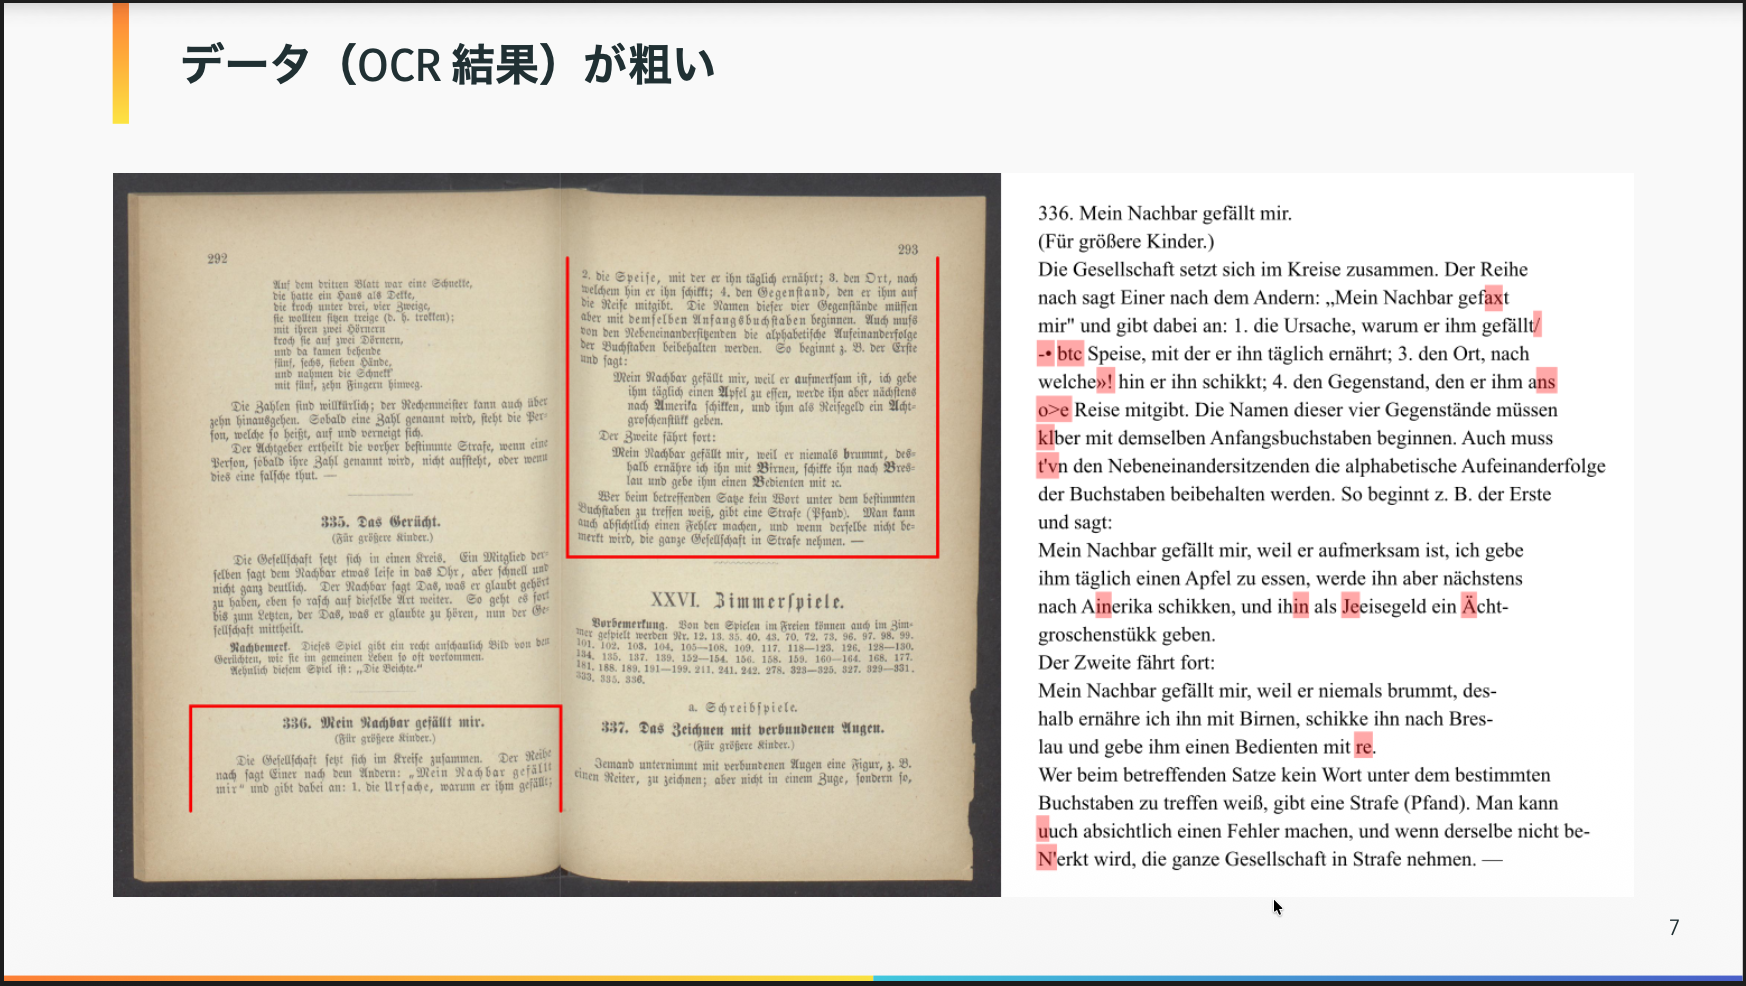
\includegraphics[width=\linewidth]{./img/spring_presentation_slide.png}
            \captionsetup{skip=-1pt}
            \caption{\fontsize{4pt}{5pt}\selectfont \texttt{\url{github.com/IllDepence/search-engineering-tech-talk-2026-spring}}}
        \end{center}
        \end{figure}
    \end{column}
    \end{columns}
\end{frame}

\begin{frame}[t]{Helpfeel社}
    \begin{columns}[T,onlytextwidth]
    \begin{column}{0.42\textwidth}
        \vskip.5em
        ナレッジの管理と活用
        \begin{itemize}
            \item 企業のナレッジを集約・管理
            \item カスタマーサポートや\newline 社内ヘルプデスクで活用
        \end{itemize}
        \onslide<2->{
        \vskip1em
        今日の話
        \begin{itemize}
            \item Helpfeel（プロダクト）
        \end{itemize}
        }
    \end{column}
    \begin{column}{0.55\textwidth}
        \begin{figure}
        \begin{center}
            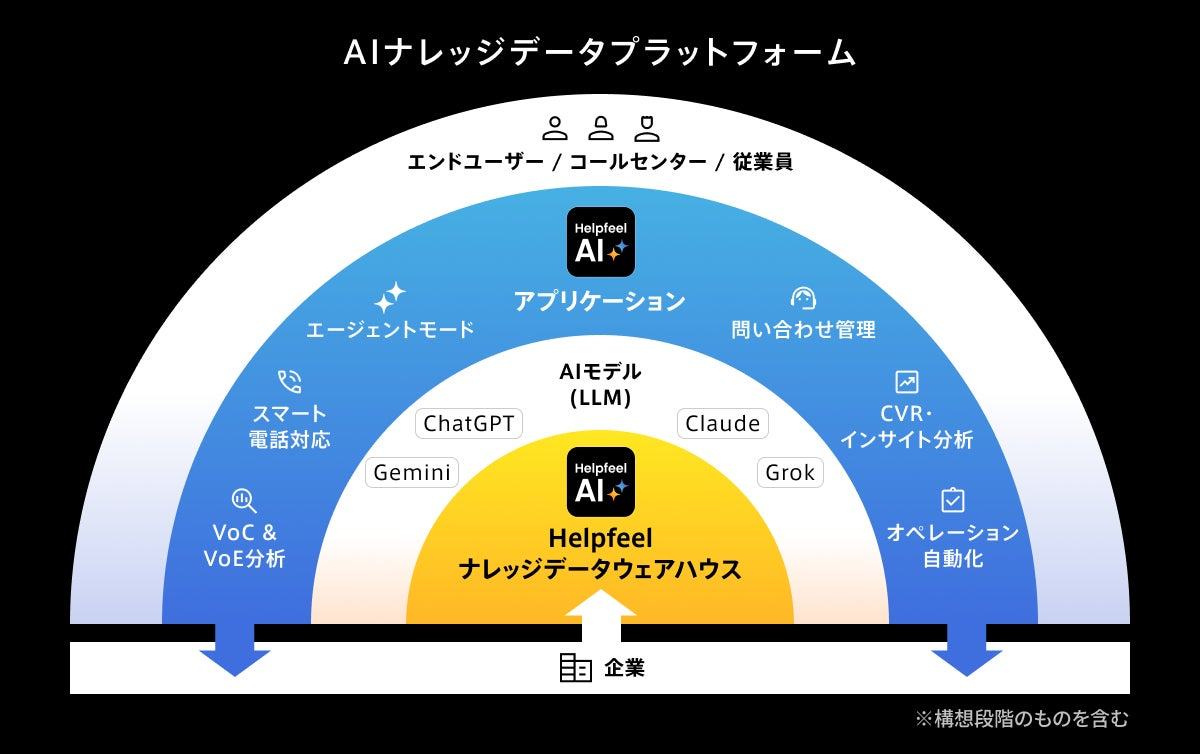
\includegraphics[width=\linewidth]{./img/helpfeel_ai_knowledge_platform.jpeg}
        \end{center}
        \end{figure}
    \end{column}
    \end{columns}
\end{frame}

\begin{frame}[t]{Helpfeel（プロダクト）}
    \only<1>{
        \vskip1em
        \begin{center}
            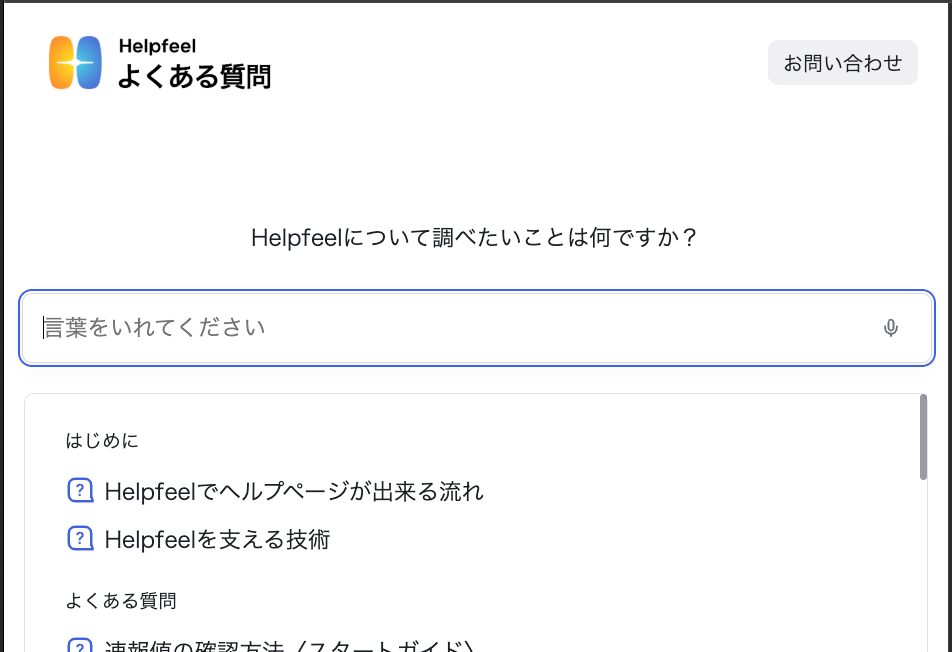
\includegraphics[height=.75\textheight]{./img/helpfeel_search_0_start.png}
        \end{center}
    }
    \only<2->{
    \begin{columns}[T,onlytextwidth]
    \begin{column}{0.43\textwidth}
        \vskip.5em
        利用シーンに応じた様々な検索
        \begin{itemize}
            \onslide<3->{\item 例1：想定質問の検索
            \begin{itemize}
                \item インクリメンタル検索
                \onslide<4->{\item ベクトル検索}
            \end{itemize}}
            \onslide<5->{\item 例2：Agentic RAG
            \begin{itemize}
                \item 今日の話題
            \end{itemize}}
        \end{itemize}
    \end{column}
    \begin{column}{0.54\textwidth}
        \begin{overprint}
            \only<3>{
                \begin{figure}
                \begin{center}
                    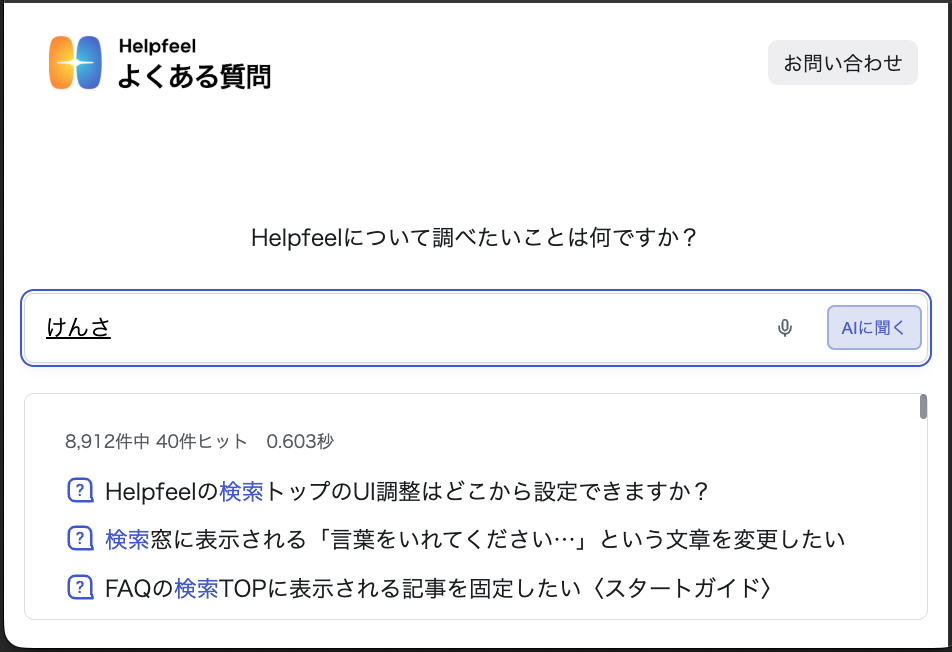
\includegraphics[width=\linewidth]{./img/helpfeel_search_0_instant.png}
                \end{center}
                \end{figure}
            }
            \only<4>{
                \begin{figure}
                \begin{center}
                    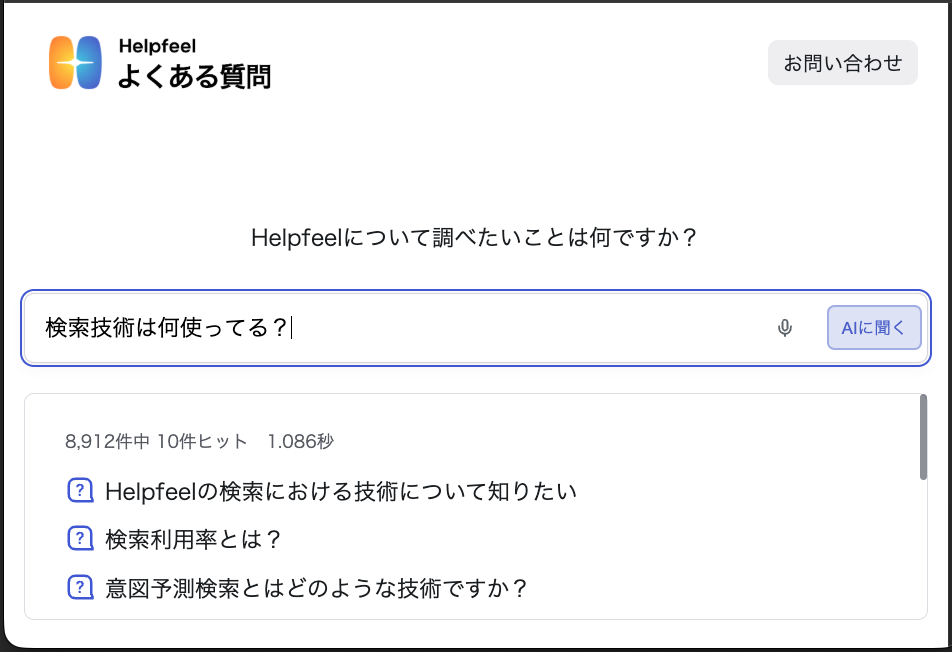
\includegraphics[width=\linewidth]{./img/helpfeel_search_1_vector.png}
                \end{center}
                \end{figure}
            }
            \only<5>{
                \begin{figure}
                \begin{center}
                    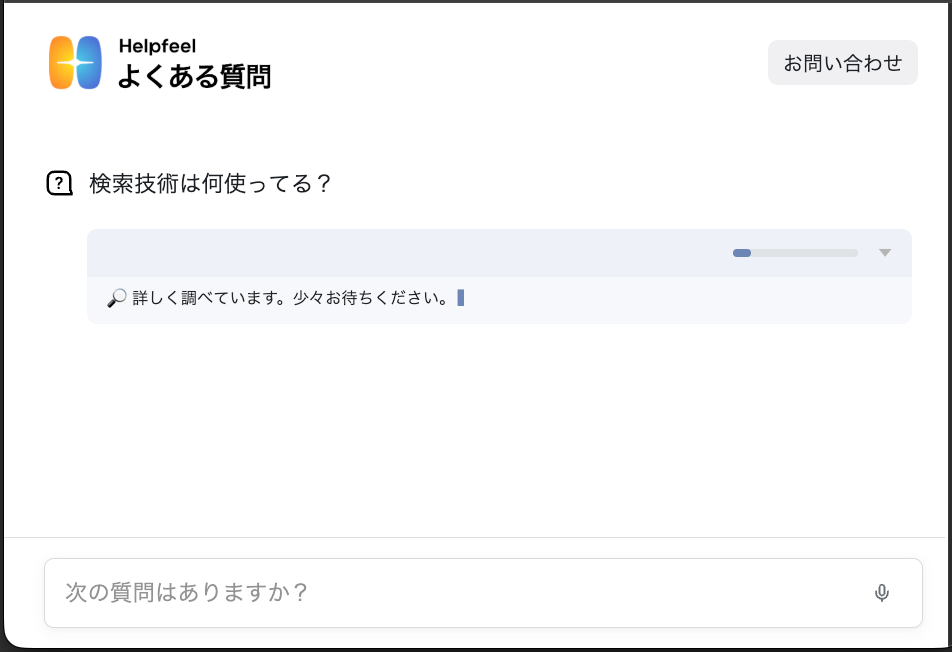
\includegraphics[width=\linewidth]{./img/helpfeel_search_2_agent_progress_e2.png}
                \end{center}
                \end{figure}
            }
            \only<6>{
                \begin{figure}
                \begin{center}
                    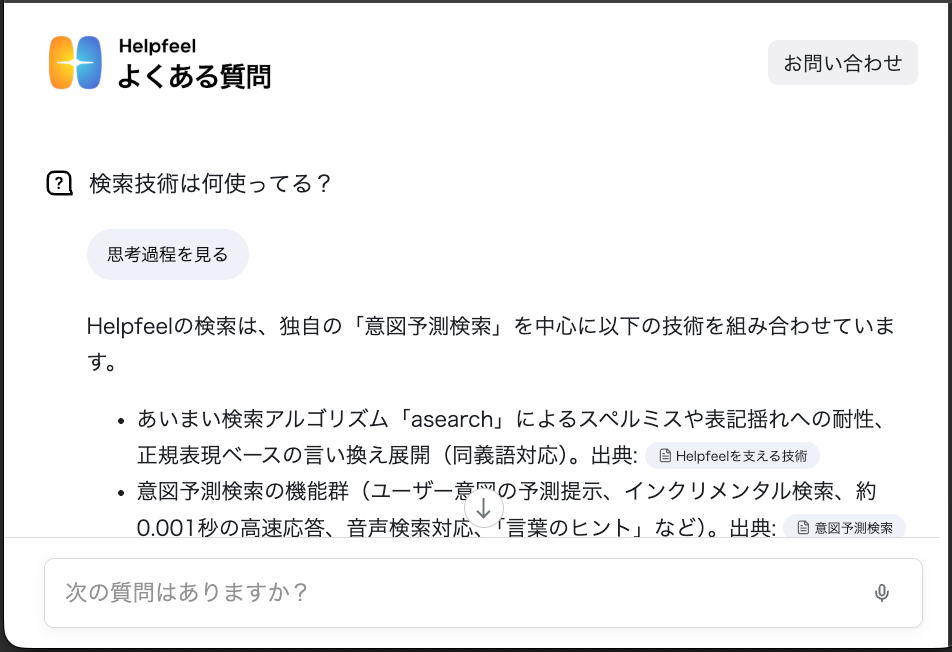
\includegraphics[width=\linewidth]{./img/helpfeel_search_3_agent_answer_e2.png}
                \end{center}
                \end{figure}
            }
        \end{overprint}
    \end{column}
    \end{columns}
    }
\end{frame}

\begin{frame}[t]{本題：Agentic RAG（Helpfeel Agent Mode）}
    \begin{columns}[T,onlytextwidth]
    \begin{column}{0.4\textwidth}
        \vskip.5em
        \begin{itemize}
            \item 様々なソースを検索して回答
            \onslide<2->{\item 当初：「じっくり検索」
            \begin{itemize}
                \item 回答できるまで検索
                \item 複数ソースを組み合わせる
            \end{itemize}}
            \onslide<3->{\item しかし：求められたのは速さ
            \begin{itemize}
                \item すぐに答えがほしい
            \end{itemize}}
        \end{itemize}
    \end{column}
    \begin{column}{0.57\textwidth}
        \vskip1.2em
        \centering
        \begin{tikzpicture}[
            src/.style={rounded corners=5pt, fill=convo-tool, minimum height=.5cm, text width=3.35cm,
                        align=center, font=\scriptsize, inner sep=1pt},
          ]
          \node (user) at (0,0) {
\includegraphics[height=.75cm]{./img/icon_user.png}};
          \node (agent) at (2.1,0) {
\includegraphics[height=.62cm]{./img/icon_bot.png}};
          \draw[flow] ([yshift=5pt]user.east) -- node[lbl, above] {質問} ([yshift=5pt]agent.west);
          \draw[flow] ([yshift=-5pt]agent.west) -- node[lbl, below] {回答} ([yshift=-5pt]user.east);
          \foreach \t [count=\i] in {ナレッジベース, PDF・Officeファイル, Web, SharePoint, \dots} {
            \node (h\i) at (3.75, 1.86-\i*0.62) {
\includegraphics[height=.38cm]{./img/icon_search.png}};
            \node[src, right=2pt of h\i] {\t};
            \draw[{Stealth[length=3pt]}-{Stealth[length=3pt]}, draw=black!35, line width=.5pt] (agent.east) -- (h\i.west);
          }
          \node[lbl] at (3.75, 1.75) {検索ツール};
        \end{tikzpicture}
    \end{column}
    \end{columns}
\end{frame}

\begin{frame}[t]{高速化プロジェクト}
    \begin{itemize}
        \item 目標
        \begin{itemize}
            \item 応答速度を上げる
            \item 検索品質とコストは維持
        \end{itemize}
        \onslide<2->{\item 課題
        \begin{itemize}
            \item 速度と品質の両立
            \item 利用顧客はまだ少ない $\rightarrow$ 今後の使われ方の予測が難しい
            \item ...
        \end{itemize}}
    \end{itemize}
\end{frame}

\begin{frame}[t]{ネタバレ}
    % no brace group around the overlays here: with metropolis it breaks beamer's overlay counting
    \centering
    \begin{tikzpicture}
        \node[anchor=south west, inner sep=0] (plot) at (0,0) {%
            \only<1>{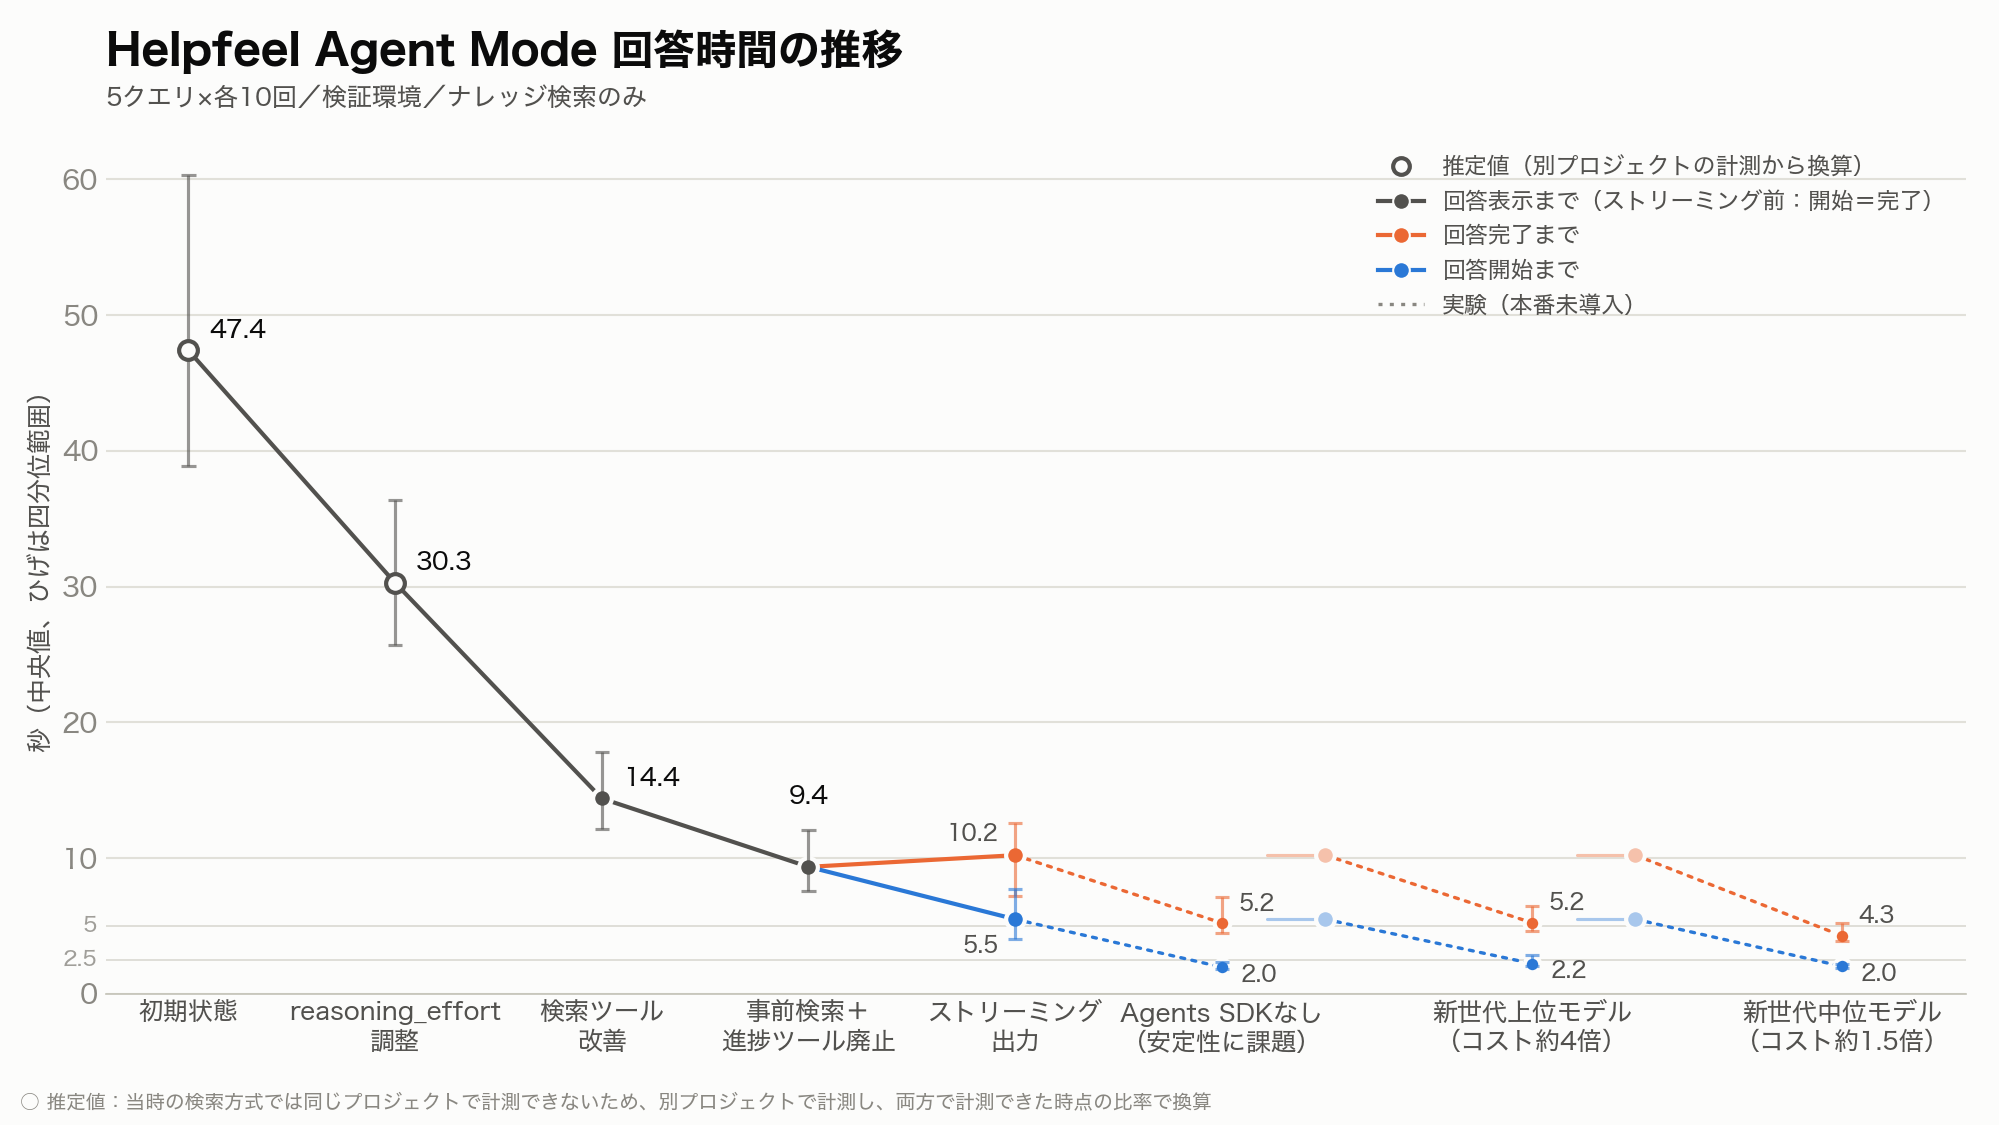
\includegraphics[height=.83\textheight]{./img/agent_mode_speedup_progression_simple_master-morning_nofill.png}}%
            \only<2->{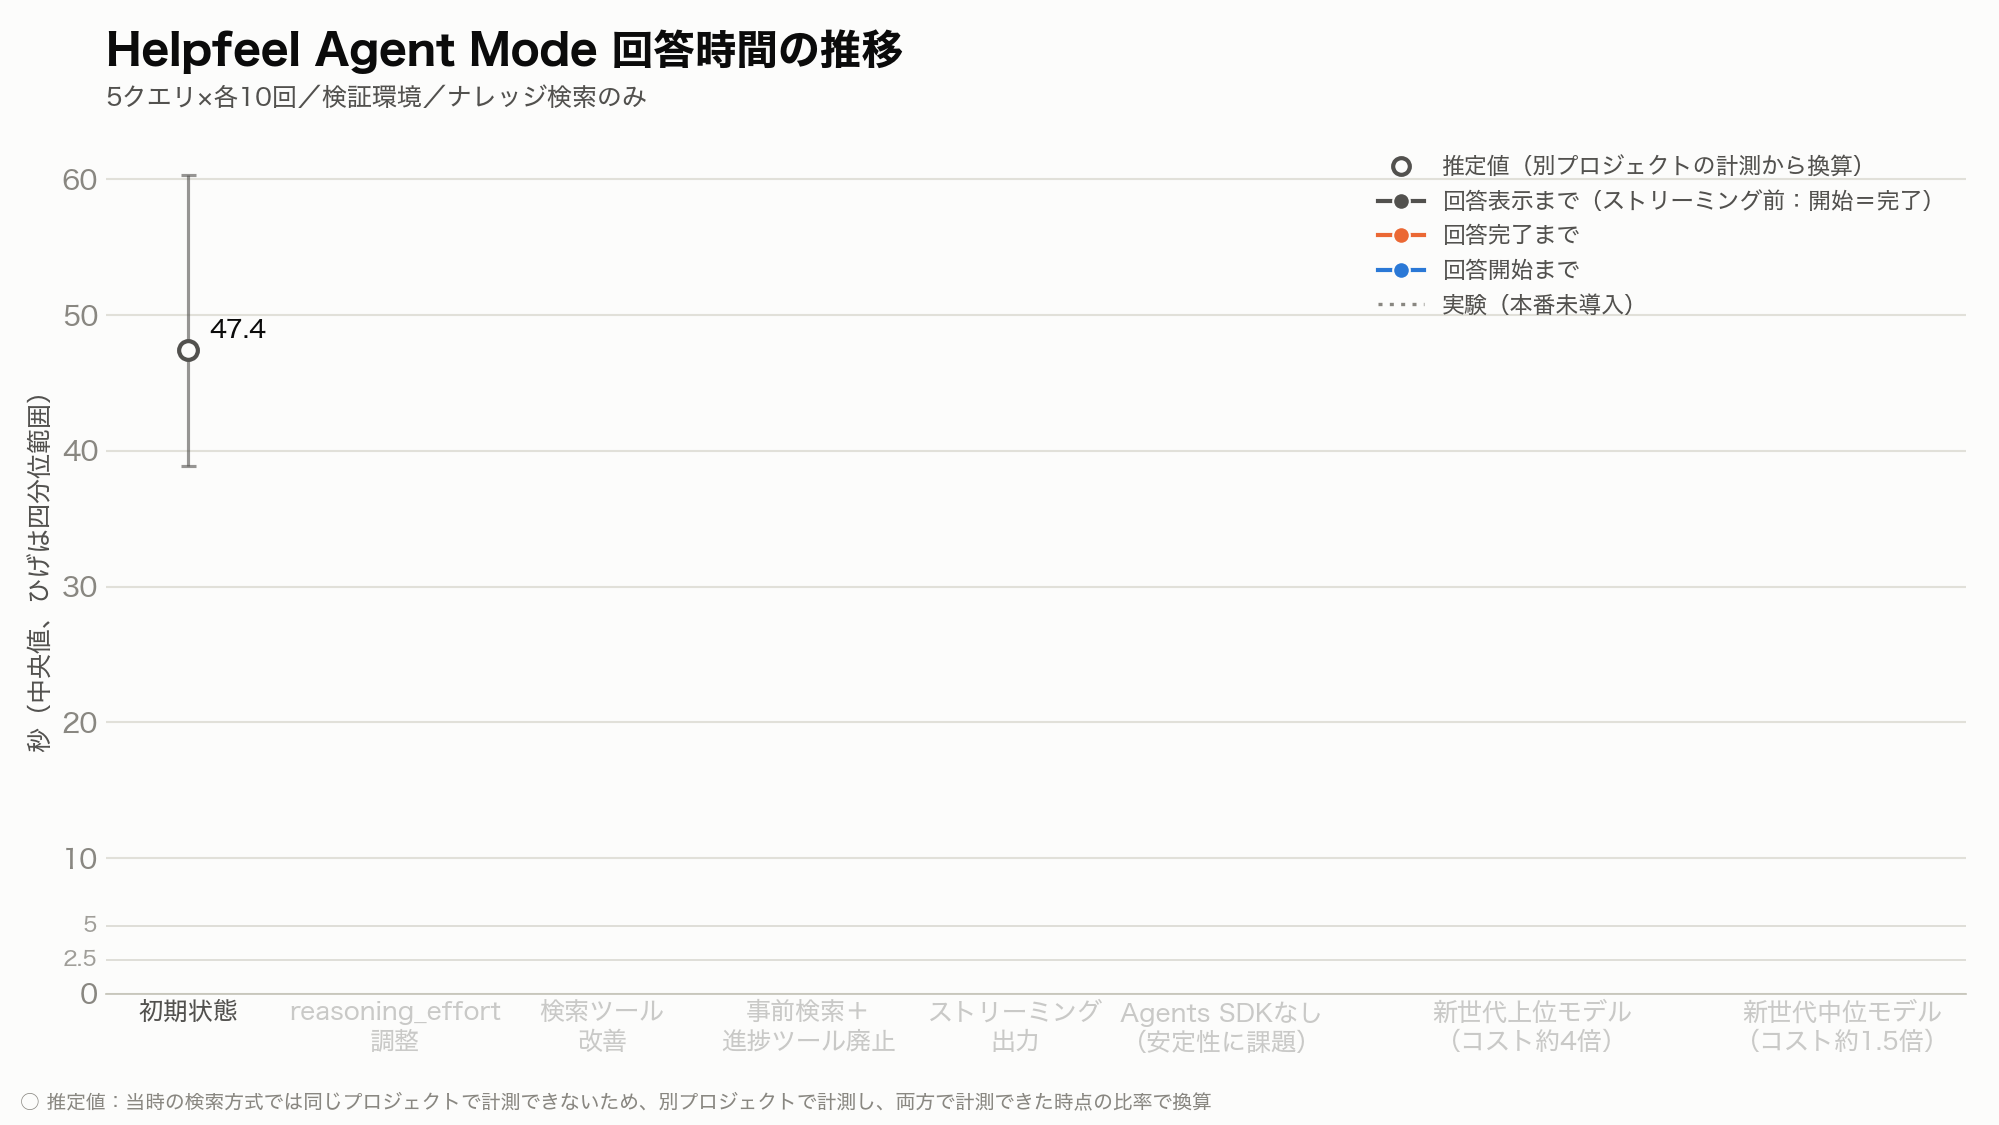
\includegraphics[height=.83\textheight]{./img/agent_mode_speedup_progression_simple_master-morning_nofill_stage1.png}}};
        % boxes in fractions of the image, from matplotlib's extents of the elements (+9 px padding)
        \begin{scope}[x={(plot.south east)}, y={(plot.north west)},
                      box/.style={draw=highlight, line width=1.5pt, rounded corners=2pt}]
            \only<3>{\draw[box] (0.0101,0.3233) rectangle (0.0312,0.6726);}  % y axis label
            \only<4>{\draw[box] (0.0483,0.8935) rectangle (0.3283,0.9309);}  % subtitle
            \only<5>{\draw[box] (0.0647,0.0807) rectangle (0.1237,0.1181);}  % x tick 初期状態
            \only<6>{\draw[box] (0.0859,0.5781) rectangle (0.1024,0.8520);}  % first point with whiskers (4 px less side padding: clear of the value label)
        \end{scope}
    \end{tikzpicture}
\end{frame}

\begin{frame}[t]{第一歩：モデルパラメータの調整}
    \only<1-3>{
    \begin{columns}[T,onlytextwidth]
    \begin{column}{0.55\textwidth}
        \vskip.5em
        APIパラメータを1つずつ変えて計測※
        \begin{valuelist}
            % measured 100/75/54/40/31 s, mapped linearly from 100-31 s to 50-31 s (see footnote)
            \vitem{既定（現行モデル）}{50秒}
            \vitem{小型モデル}{43秒}
            \vitem{verbosity low}{37秒}
            \vitem{parallel\_tool\_calls}{33秒}
            \vitem[\onslide<2->{\,\cmark}]{reasoning\_effort low}{31秒}
        \end{valuelist}
    \end{column}
    \begin{column}{0.4\textwidth}
        \vskip.5em
        \onslide<2->{
        reasoning\_effort low
        \begin{itemize}
            \item 品質は十分
            \item 単独で最大の効果
        \end{itemize}
        }
        \onslide<3->{
        \vskip1em
        $\rightarrow$「思考レベル」設定
        \begin{itemize}
            \item シンプル（low）
            \item バランス（medium）
            \item じっくり（high）
            \item デフォルト：シンプル
        \end{itemize}
        }
    \end{column}
    \end{columns}
    \vfill
    {\scriptsize ※ 回答時間の推移（グラフ）とは別の検証環境・シナリオでの計測（数値は換算値）}
    }
    \only<4>{\progressionplot{_stage1}}  % before
    \only<5>{\progressionplot{_stage2}}  % after
\end{frame}

\begin{frame}[t]{ツール改善}
    \only<1-3>{
    ナレッジ検索ツール
    \begin{itemize}
        \item キーワード検索
        \begin{itemize}
            \item 前：キーワードでスニペットを検索
            \item 後：n-gram全文検索、ページ全体を返す
        \end{itemize}
        \onslide<2->{\item ベクトル検索を追加
        \begin{itemize}
            \item キーワード検索とのハイブリッド
        \end{itemize}}
        \onslide<3->{\item どちらも言い換えクエリでの再検索を減らす
        \begin{itemize}
            \item 検索1回が速くなったわけではない
            \item 回答までの検索回数が減る
        \end{itemize}}
    \end{itemize}
    }
    \only<4>{\progressionplot{_stage2}}  % before
    \only<5>{\progressionplot{_stage3}}  % after
\end{frame}

\begin{frame}[t]{間奏：LLMの「会話」と「ツール呼び出し」}
    \only<1>{
    \begin{itemize}
        \item 見た目：同じ相手との往復
        \item そう感じられるように組み立てられている
    \end{itemize}
    }
    \only<2>{
    \begin{itemize}
        \item 実際：返答ごとに新しいLLMインスタンス
        \item それまでのやり取り全体をコンテキストとして渡す
    \end{itemize}
    }
    \only<3>{
    \begin{itemize}
        \item ツール呼び出しも同じ仕組み
        \item 呼び出しごとにLLMとの1往復
    \end{itemize}
    }
    \only<4>{
    \begin{itemize}
        \item 往復ごとに時間がかかる（プロンプトキャッシュで軽減されるが）
        \item $\rightarrow$ ツール呼び出しを減らす
    \end{itemize}
    }
    \begin{overprint}
        \onslide<1>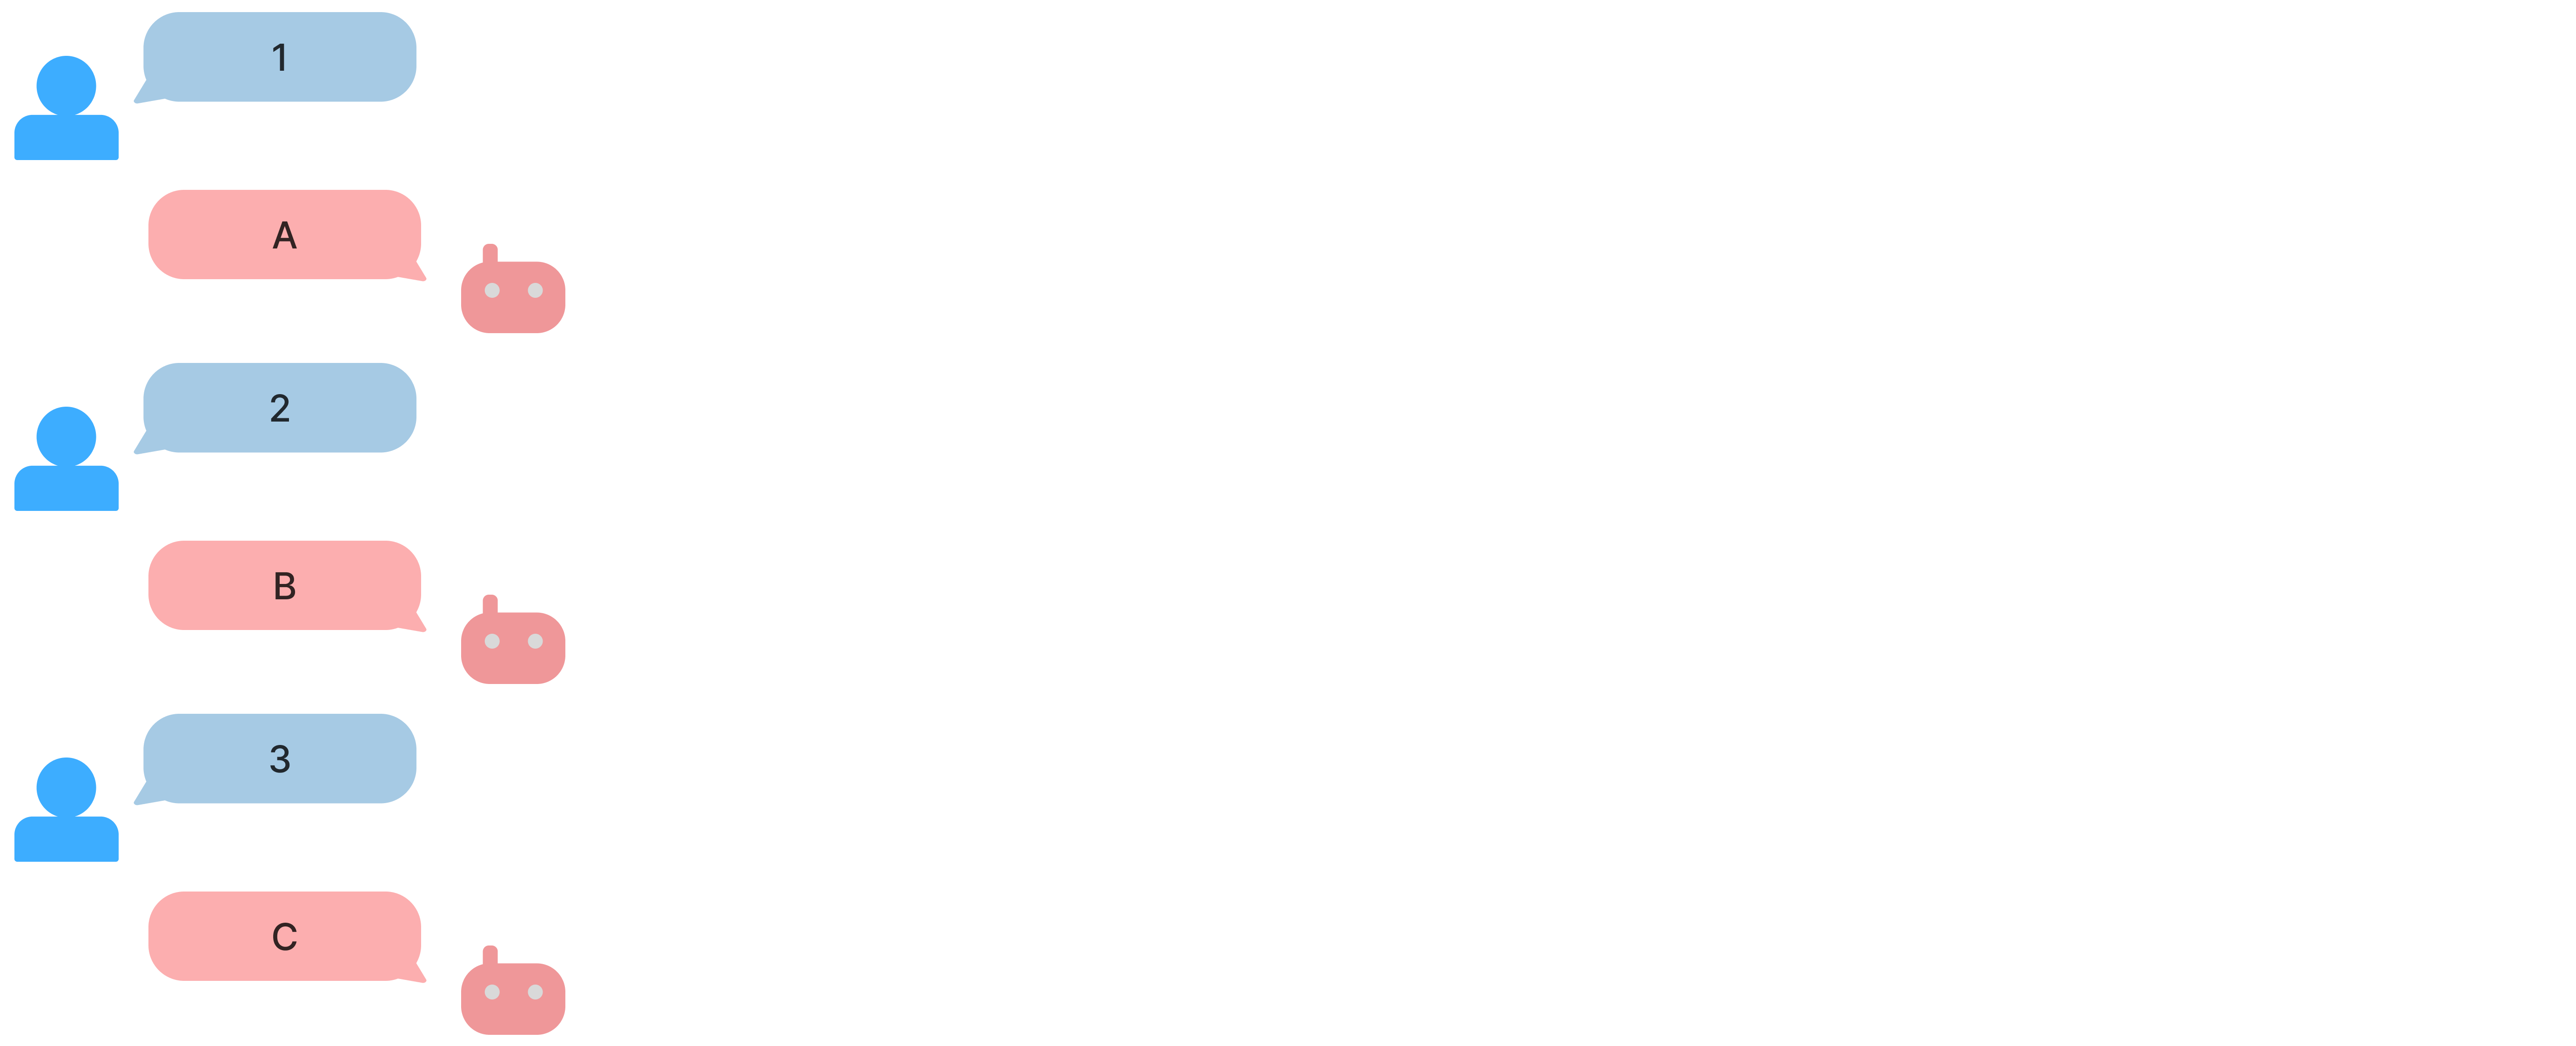
\includegraphics[width=\linewidth]{./img/llm_convo_0.png}
        \onslide<2>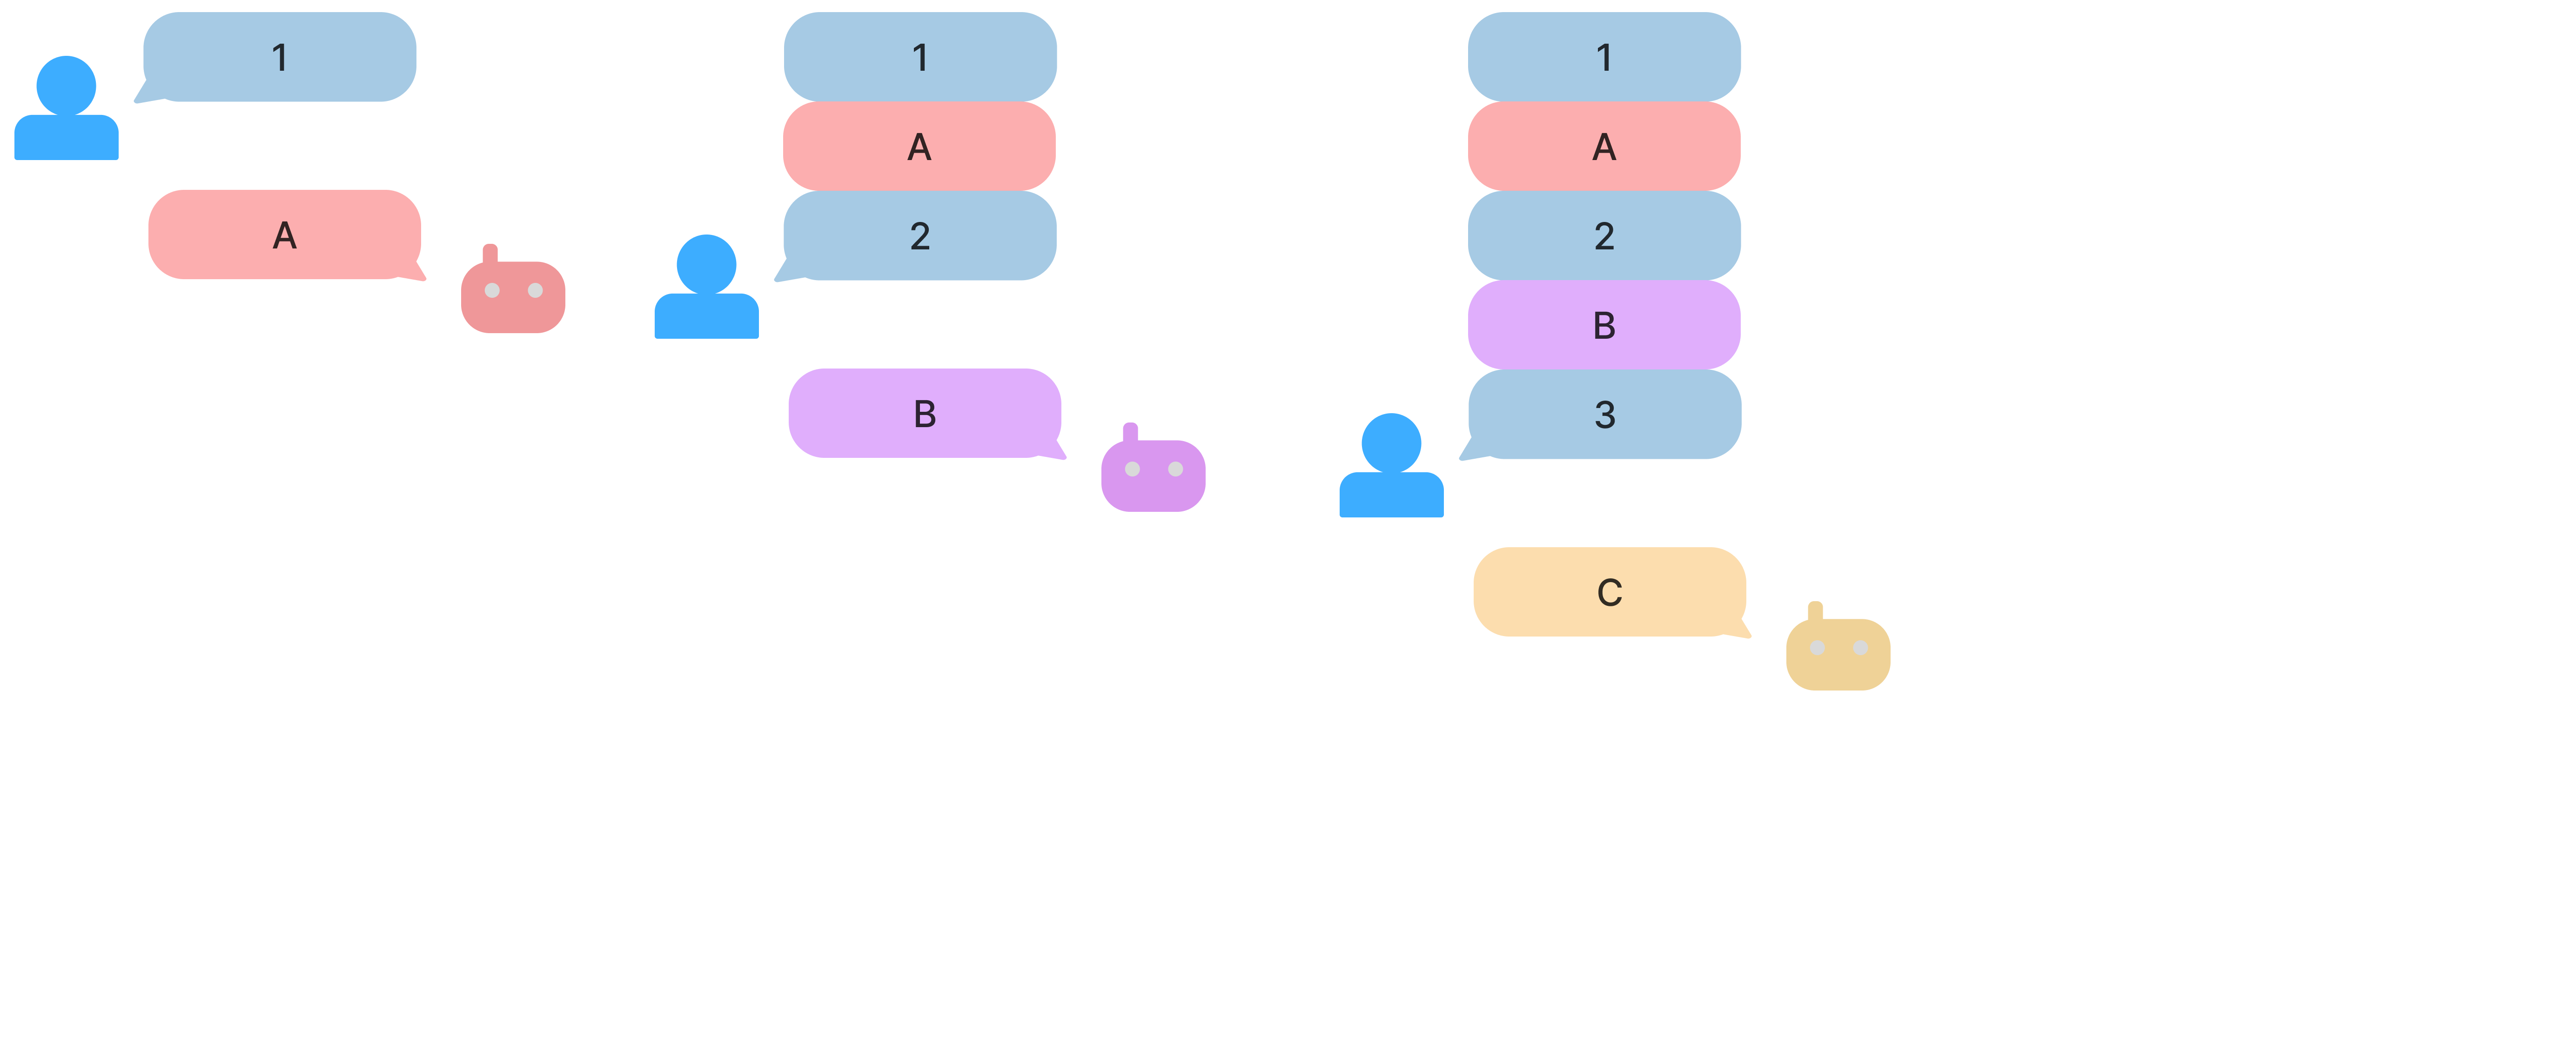
\includegraphics[width=\linewidth]{./img/llm_convo_1.png}
        \onslide<3-4>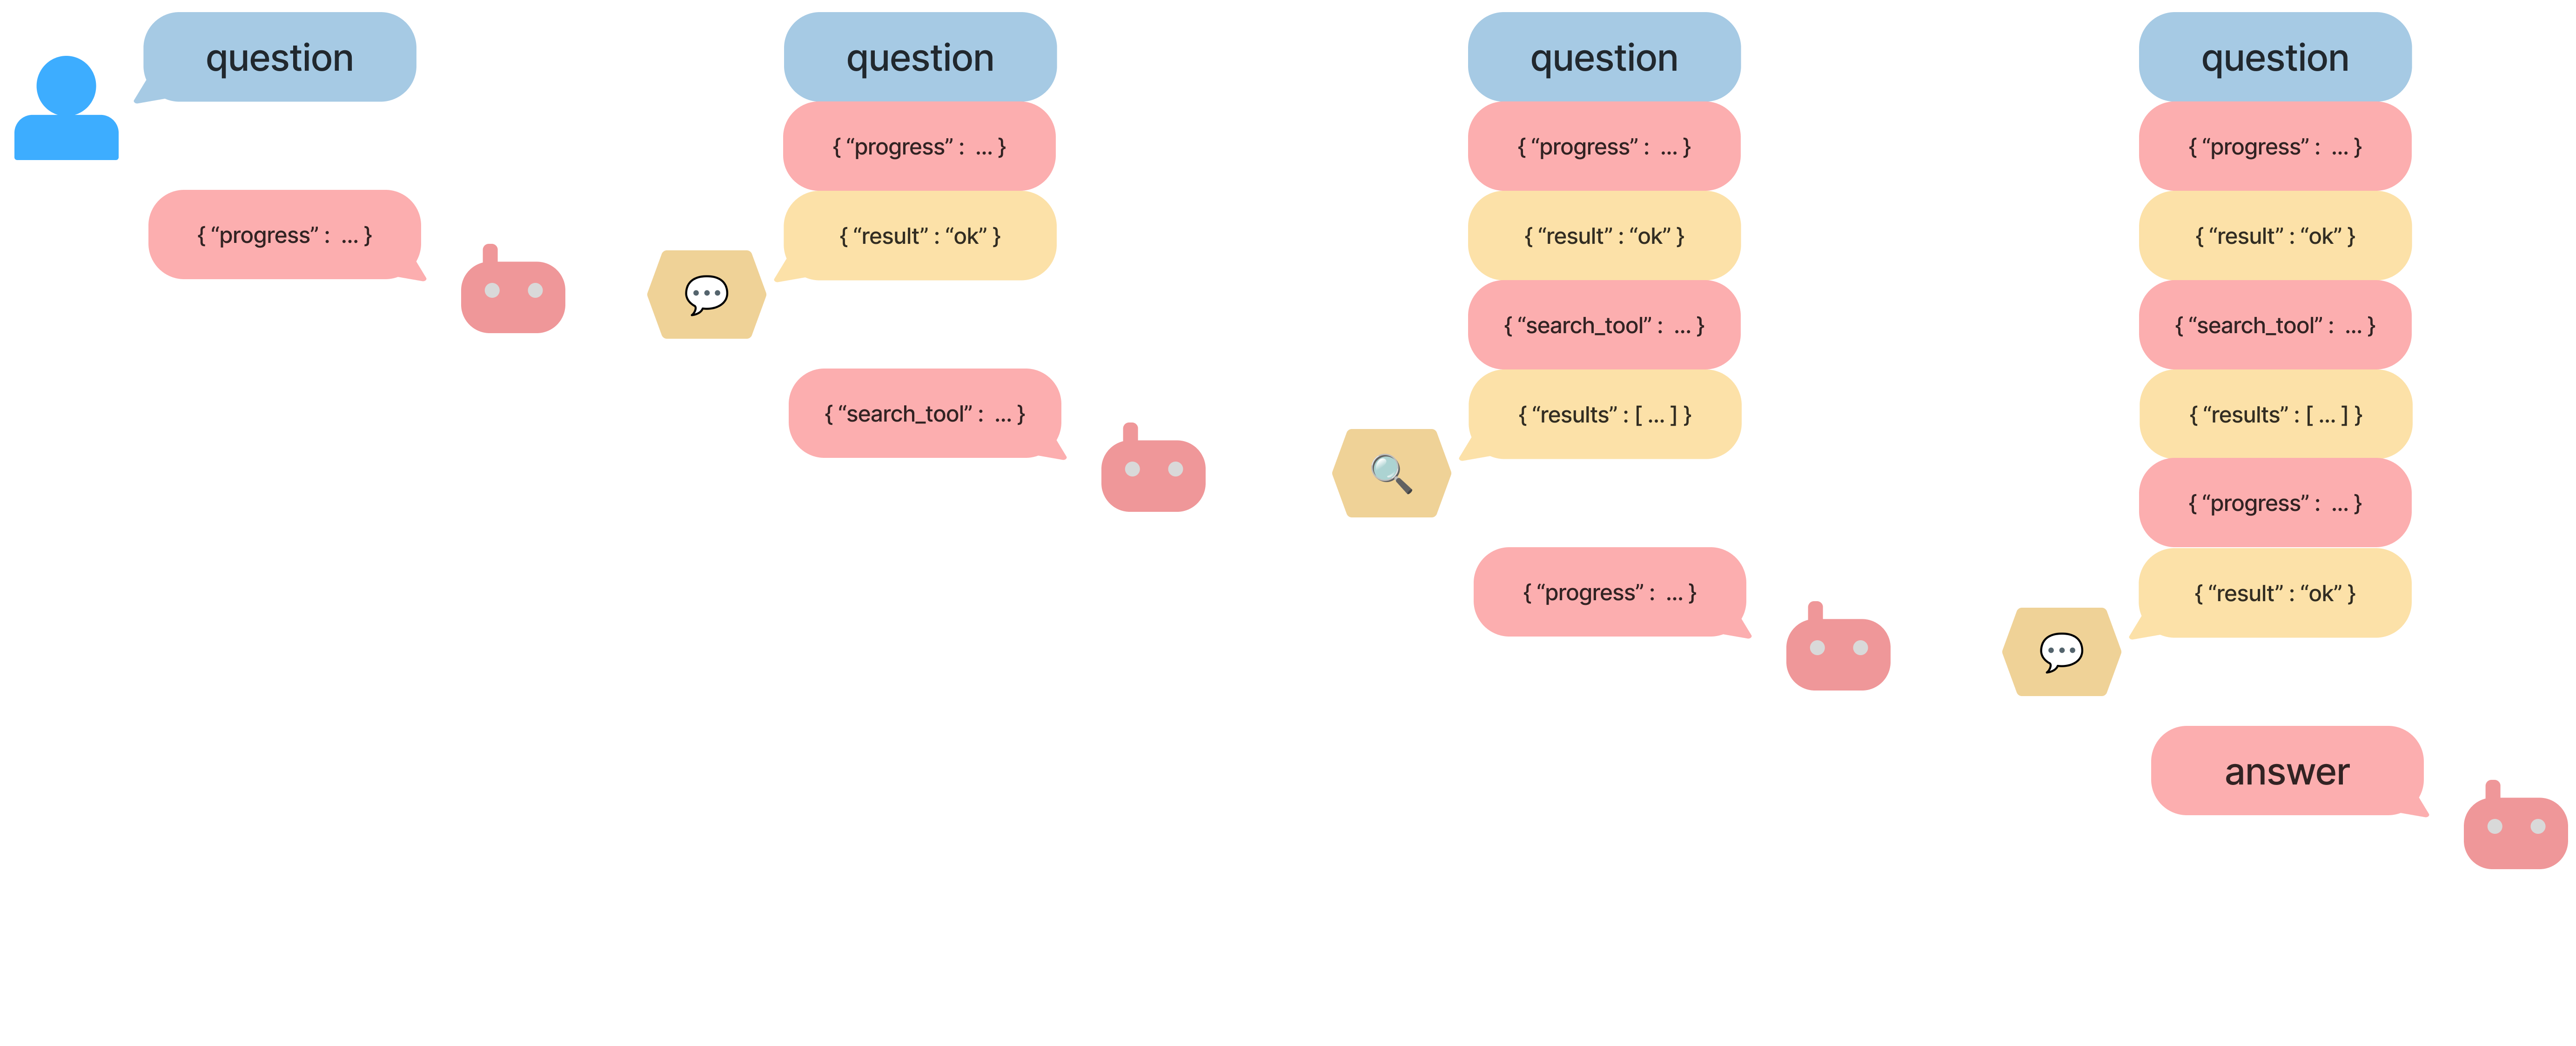
\includegraphics[width=\linewidth]{./img/llm_convo_2.png}
    \end{overprint}
\end{frame}

\begin{frame}[t]{高速化への応用}
    \only<1-4>{
    \only<1>{
    \begin{itemize}
        \item 導出過程の表示（進捗メッセージ）
        \item これまで：LLMがツールで進捗メッセージを出力
    \end{itemize}
    }
    \only<2>{
    \begin{itemize}
        \item 進捗メッセージもツール呼び出し
        \item 1回答あたり平均3.9回のツール呼び出し
    \end{itemize}
    }
    \only<3>{
    \begin{itemize}
        \item 進捗ツールを廃止（メッセージはサーバ側で生成）
        \item ツール呼び出し：平均3.9回 $\rightarrow$ 1.3回
    \end{itemize}
    }
    \only<4>{
    \begin{itemize}
        \item 事前検索：ユーザーのクエリそのままで検索
        \item ツール呼び出しなしで回答できる
    \end{itemize}
    }
    \begin{overprint}
        \onslide<1>\begin{center}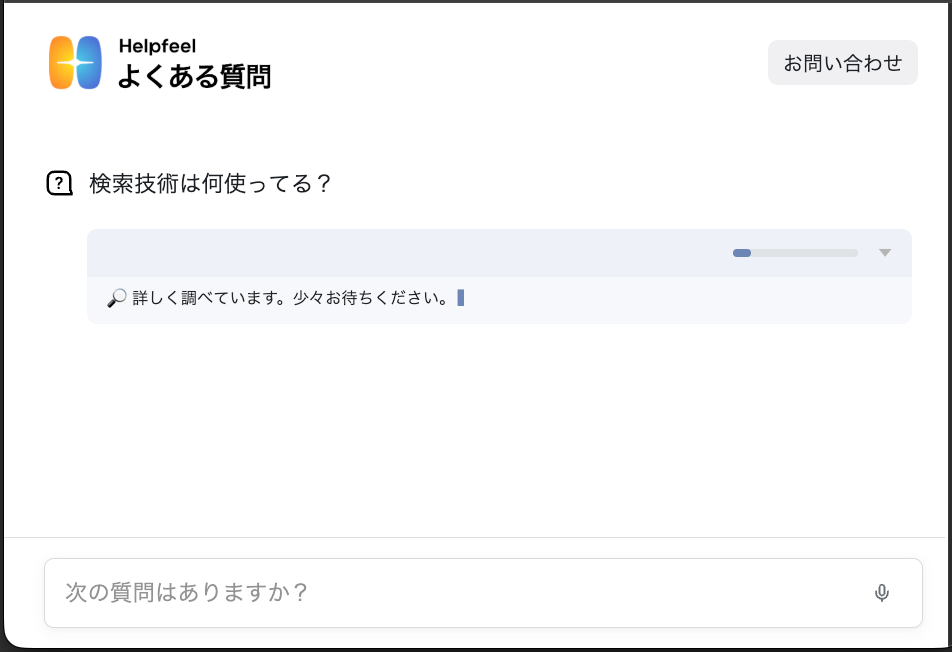
\includegraphics[height=.6\textheight]{./img/helpfeel_search_2_agent_progress_e2.png}\end{center}
        \onslide<2>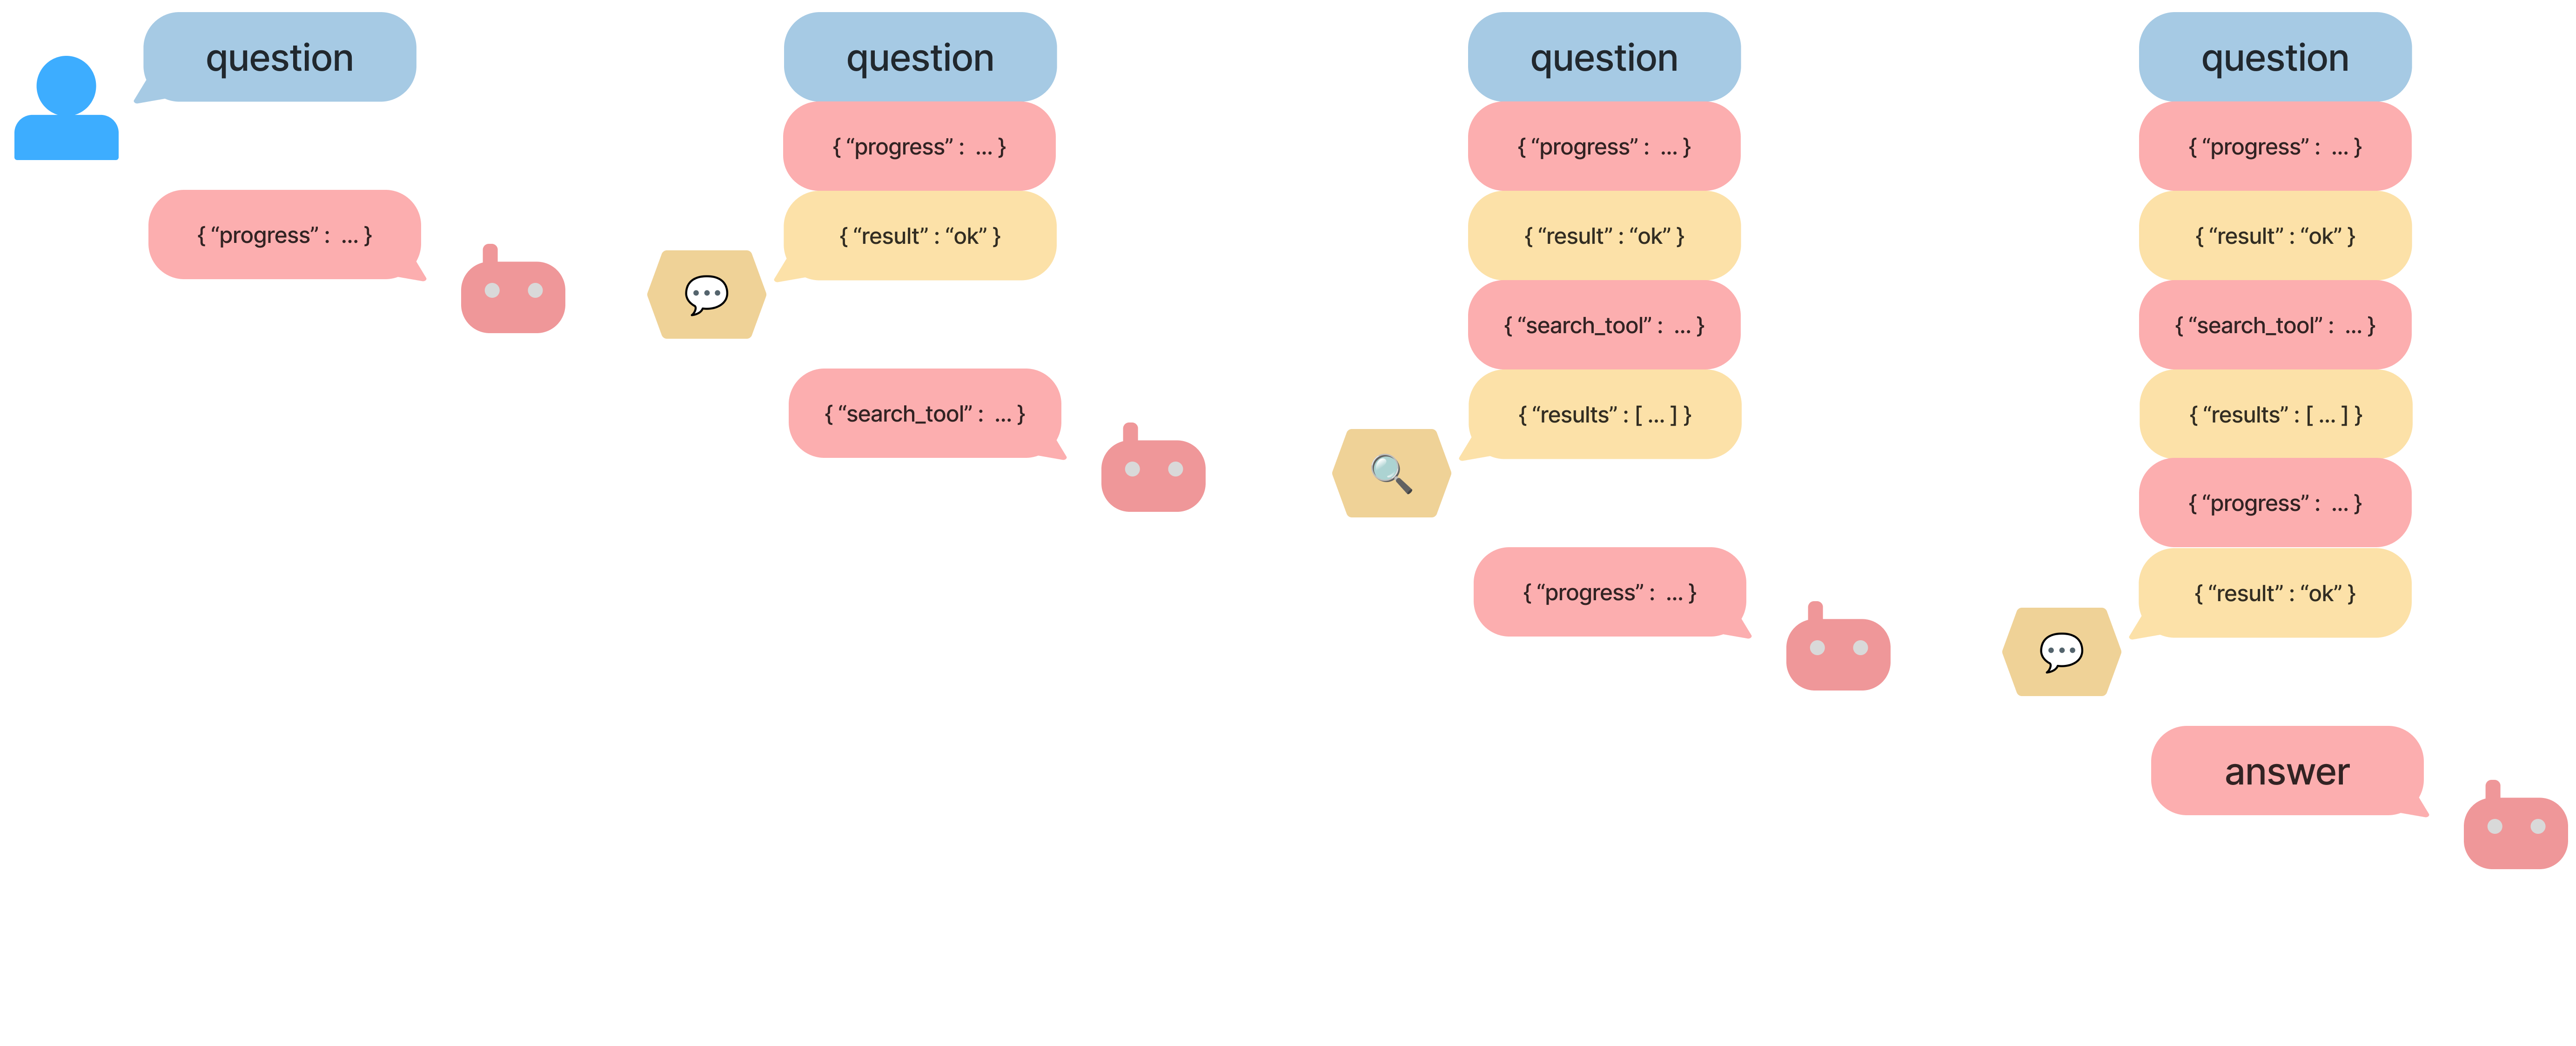
\includegraphics[width=\linewidth]{./img/llm_convo_2.png}
        \onslide<3>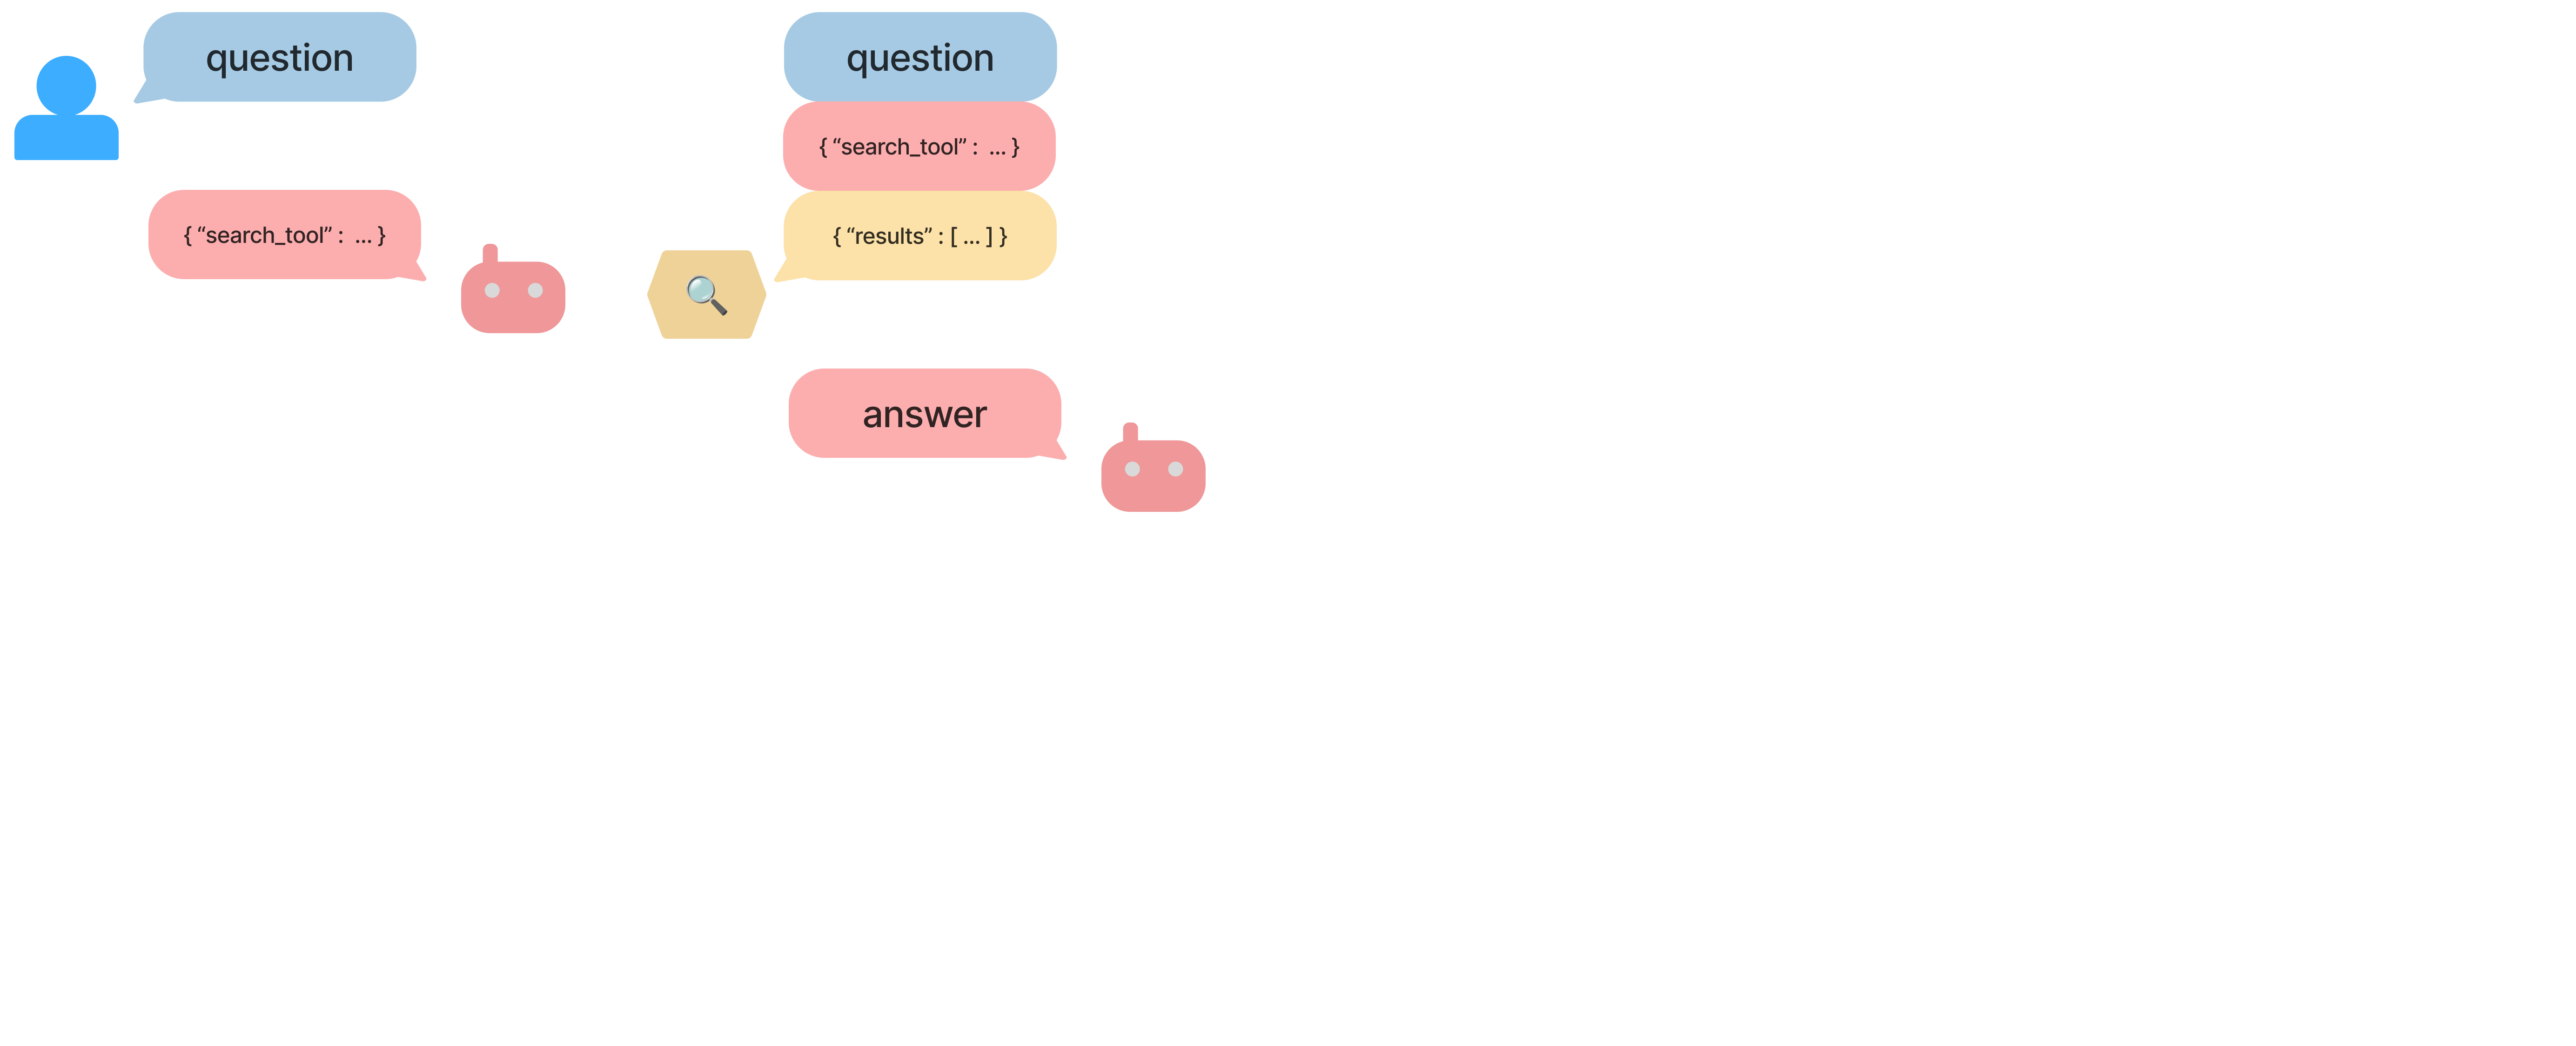
\includegraphics[width=\linewidth]{./img/llm_convo_3.png}
        \onslide<4>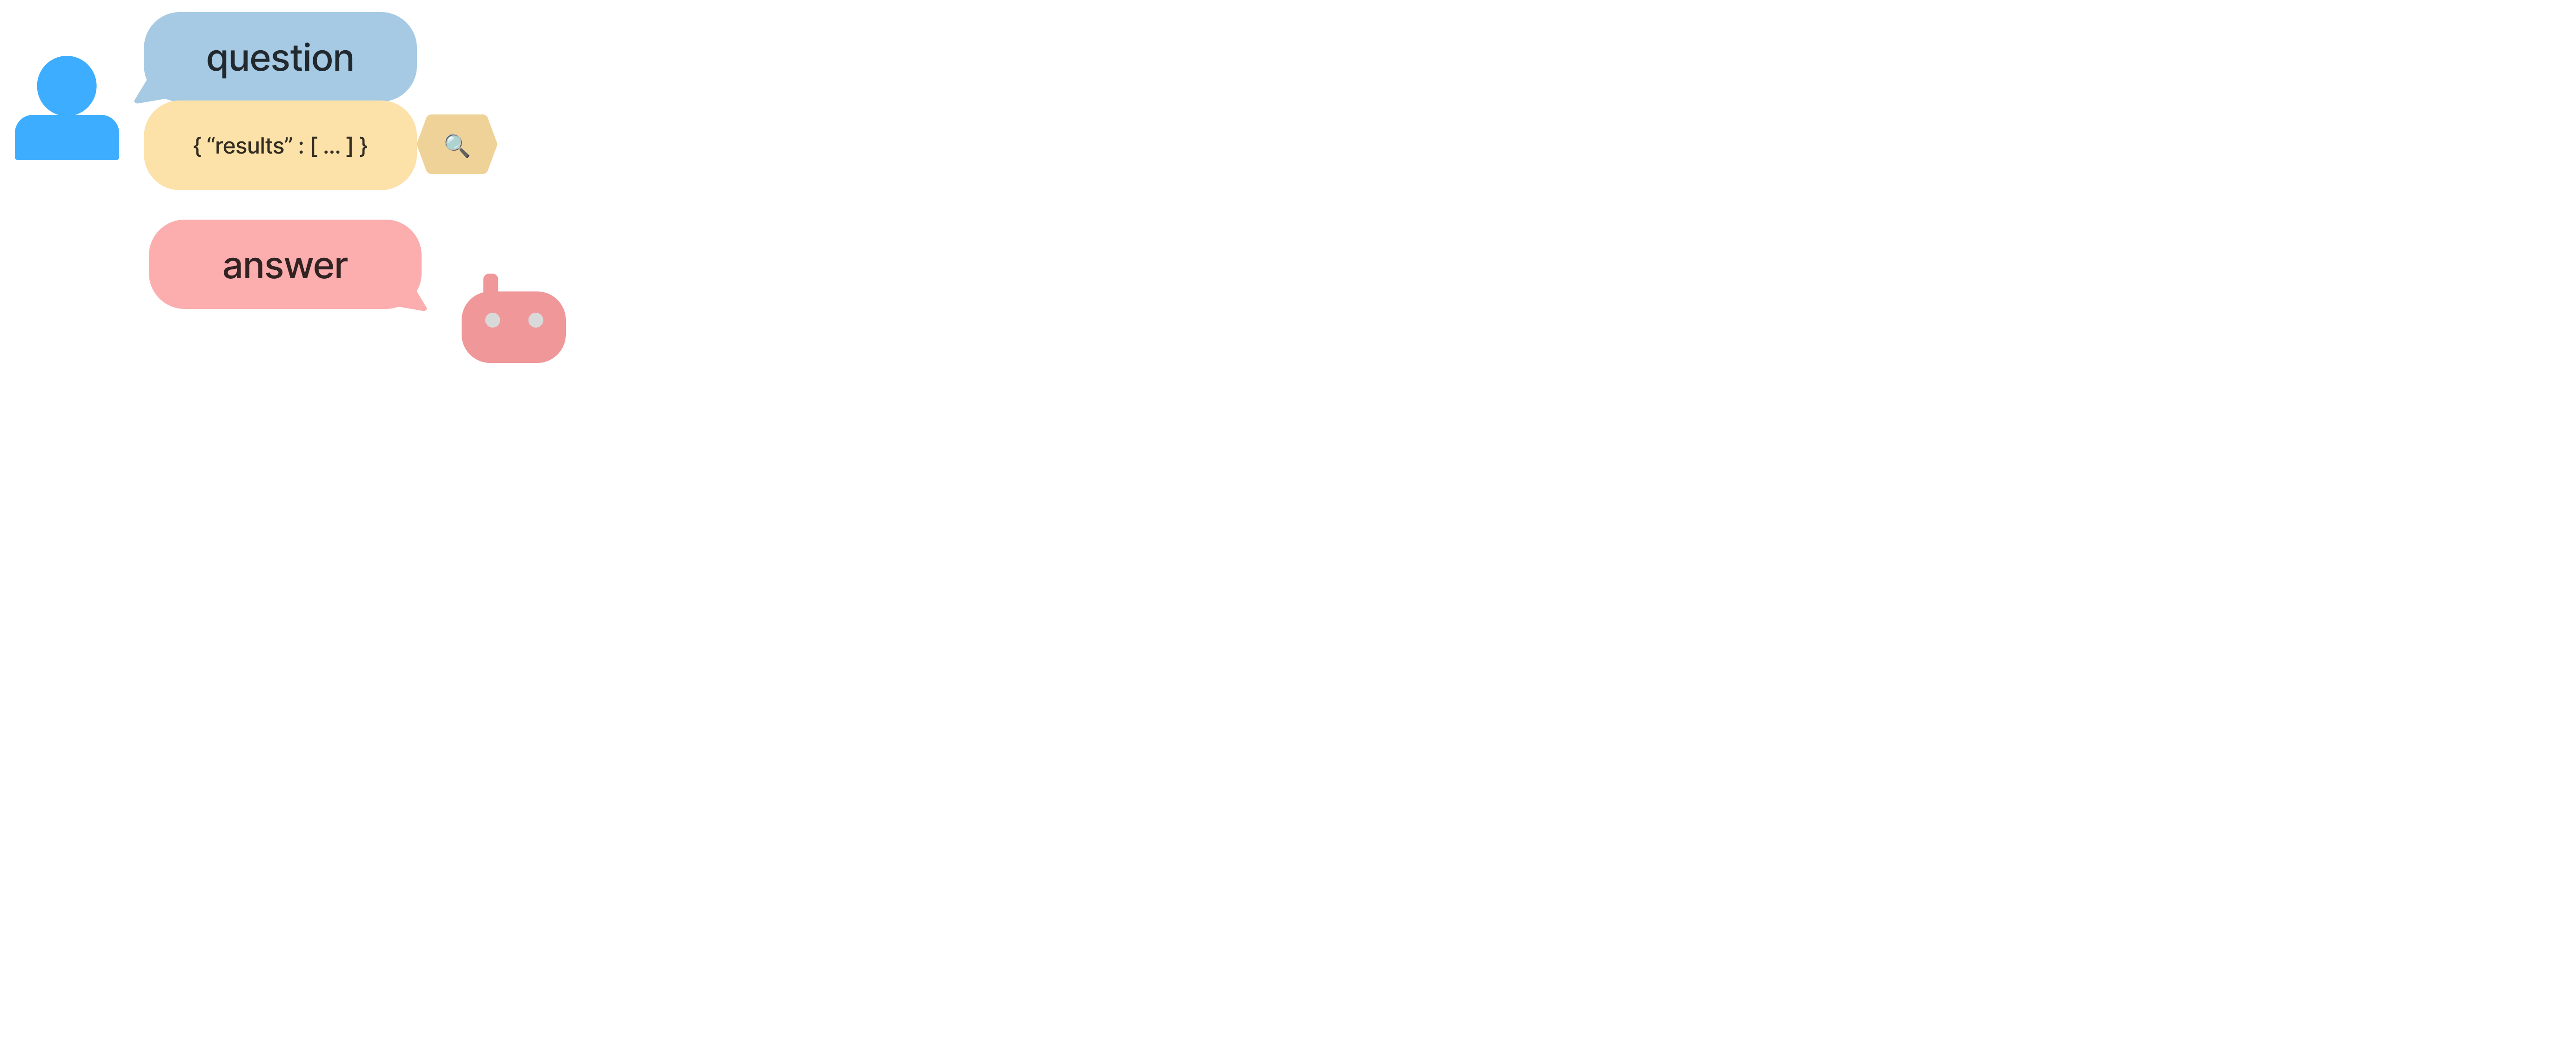
\includegraphics[width=\linewidth]{./img/llm_convo_4.png}
    \end{overprint}
    }
    \only<5>{\progressionplot{_stage3}}  % before
    \only<6>{\progressionplot{_stage4}}  % after
\end{frame}

\begin{frame}[t]{事前検索：詳細}
    \vskip.5em
    検索結果をモデルコンテキストにどう入れる？
    \begin{columns}[T,onlytextwidth]
    \begin{column}{0.48\textwidth}
        \begin{itemize}
            \item システムプロンプトに追加
            \begin{itemize}
                \item[\xmark] 毎ターン変化 $\rightarrow$ キャッシュ無効
            \end{itemize}
            \onslide<2->{\item systemメッセージとして追加
            \begin{itemize}
                \item[\xmark] 検索結果が指示扱いに
            \end{itemize}}
            \onslide<3->{\item assistantメッセージとして追加
            \begin{itemize}
                \item[\xmark] モデル自身の発言扱いに
            \end{itemize}}
        \end{itemize}
    \end{column}
    \begin{column}{0.48\textwidth}
        \begin{itemize}
            \onslide<4->{\item userメッセージとして追加（採用）
            \begin{itemize}
                \item[\cmark] API上の懸念なし
                \item[\xmark] 同じクエリで再検索のリスク
            \end{itemize}}
            \onslide<5->{\item ツール実行に見せかける（未検証）
            \begin{itemize}
                \item[\cmark] 重複検索を防ぐ
                \item[\xmark] 公開事例なし・APIエラーの恐れ
            \end{itemize}}
        \end{itemize}
    \end{column}
    \end{columns}
    \onslide<6->{
    \vskip1em
    余談：テレメトリーではどう表現？
    \begin{itemize}
        \item ツール呼び出し？　別のもの？
    \end{itemize}}
\end{frame}

\begin{frame}[t]{モデルコンテキストの工夫：トークン節約}
    \begin{itemize}
        \item 検索ツールの出力を短く
        \begin{itemize}
            \item HTML表現の最適化
            \item 検索結果1件あたりの文字数：約47\%減
        \end{itemize}
        \onslide<2->{\item 速度への効果：ほぼなし}
        \onslide<3->{\item コスト：それ自体では削減
        \begin{itemize}
            \item $\rightarrow$ より高価な（が速い）モデルを使う余地
        \end{itemize}}
        \onslide<4->{\item 当社の場合
        \begin{itemize}
            \item 検索品質向上のための別の改修が節約分を吸収
            \item $\rightarrow$ コストの上昇を防いだ
        \end{itemize}}
    \end{itemize}
\end{frame}

\begin{frame}[t]{ストリーミング出力}
    \only<1-3>{
    \begin{itemize}
        \item 回答を生成しながら表示
        \onslide<2->{\item 回答完了までの時間は変わらない}
        \onslide<3->{\item それでもユーザーは早く情報にアクセスできる}
    \end{itemize}
    }
    \only<4>{\progressionplot{_stage4}}  % before
    \only<5>{\progressionplot{_stage5}}  % after
\end{frame}

\begin{frame}[t]{見送った試み：Agents SDKなしのAgentic RAG}
    \only<1-4>{
    \begin{itemize}
        \item 事前検索だけで回答できるケースに最適化
        \onslide<2->{\item Agents SDKなし：ツールなしの普通のLLM呼び出し
        \begin{itemize}
            \item 「ツールを呼ぶか」の推論が不要
            \item ツール定義の分、入力が短い
            \item reasoning\_effort minimalが使える
        \end{itemize}}
        \onslide<3->{\item 追加の検索が必要な場合：特殊トークン（Unicodeの私用領域の文字）を出力}
        \onslide<4->{\item 見送り理由：再検索の安定性・保守の手間}
    \end{itemize}
    \onslide<2->{
    \centering
    \begin{tikzpicture}
      \node (user) at (0,0) {
\includegraphics[height=.7cm]{./img/icon_user.png}};
      \node (pre) at (2.8,0) {
\includegraphics[height=.5cm]{./img/icon_search.png}};
      \node[lbl, above=0pt of pre] {事前検索};
      \node (llm) at (5.6,0) {
\includegraphics[height=.58cm]{./img/icon_bot.png}};
      \node[lbl, above=0pt of llm] {LLM（minimal）};
      \node[rounded corners=5pt, fill=convo-bot, font=\scriptsize, minimum height=.5cm, inner xsep=6pt] (ans) at (9.4,0) {回答をストリーミング};
      \draw[flow] (user) -- node[lbl, below] {質問} (pre);
      \draw[flow] (pre) -- node[lbl, below] {検索結果} (llm);
      \draw[flow] (llm) -- (ans);
      \onslide<3->{
        \node (re) at (5.6,-1.5) {
\includegraphics[height=.5cm]{./img/icon_search.png}};
        \node[lbl, right=1pt of re] {追加検索（最大2回）};
        \draw[flow] ([xshift=-6pt]llm.south) -- node[lbl, left] {特殊トークン} ([xshift=-6pt]re.north);
        \draw[flow] ([xshift=6pt]re.north) -- node[lbl, right] {検索結果} ([xshift=6pt]llm.south);
      }
    \end{tikzpicture}
    }
    }
    \only<5>{\progressionplot{_stage5}}  % before
    \only<6>{\progressionplot{_stage6}}  % after
\end{frame}

\begin{frame}[t]{モデル変更の検討}
    \only<1-2>{
    \begin{itemize}
        \item 新世代上位モデル
        \begin{itemize}
            \item 回答開始まで：約6割短縮
            \item コスト：約4倍 $\rightarrow$ 不採用
        \end{itemize}
        \onslide<2->{\item （さらに）新世代中位モデル
        \begin{itemize}
            \item 回答開始まで：約6割短縮
            \item コスト：約1.5倍
            \item 品質・スタイル面の懸念
            \item $\rightarrow$ 全体の切り替えは見送り
            \item $\rightarrow$ プロジェクト単位の選択肢として検討中
        \end{itemize}}
    \end{itemize}
    }
    \only<3>{\progressionplot{_stage6}}  % before
    \only<4>{\progressionplot{}}  % after
\end{frame}

\begin{frame}[t]{検索品質の担保}
    \begin{itemize}
        \item 高速化で検索品質が落ちていないかの確認
        \item $\rightarrow$ 今後の発表テーマ？
    \end{itemize}
\end{frame}

\begin{frame}[t]{まとめ}
    \begin{columns}[T,onlytextwidth]
    \begin{column}{0.5\textwidth}
        \vskip.5em
        工夫と効果\\
        {\scriptsize 回答表示までの時間の短縮率}
        \begin{valuelist}
            \vitem{reasoning\_effort調整}{$-$36\%}
            \vitem{検索ツール改善}{$-$52\%}
            \vitem{事前検索＋進捗ツール廃止}{$-$35\%}
            \vitem{ストリーミング出力}{$-$41\%}
            \noalign{\vskip.3em}
            & 全体 & $-$88\% & \\
        \end{valuelist}
        {\scriptsize （回答完了までは$-$78\%）}
    \end{column}
    \begin{column}{0.47\textwidth}
        \vskip.5em
        \onslide<2->{
        教訓
        \begin{itemize}
            \item LLMとの往復を減らす
            \item 体感速度も大事
            \item トークン節約 $\rightarrow$ モデル選択の余地
            \item 応答速度とのトレードオフ
            \begin{itemize}
                \item コスト
                \item 品質
                \item 安定性
            \end{itemize}
        \end{itemize}
        }
    \end{column}
    \end{columns}
\end{frame}

\begin{frame}[t]{ご清聴ありがとうございました}
    tarek（タレク）\\
    株式会社Helpfeel
    \begin{columns}
    \begin{column}{0.3\textwidth}
        \begin{center}
        \begin{figure}
        
\includegraphics[width=0.7\textwidth]{./img/qr_github.png}
        \end{figure}
        \footnotesize\texttt{github.com/IllDepence}
        \end{center}
    \end{column}
    \begin{column}{0.3\textwidth}
        \begin{center}
        \begin{figure}
        
\includegraphics[width=0.7\textwidth]{./img/qr_hf_recruit.png}
        \end{figure}
        \footnotesize\texttt{Helpfeel 採用情報}
        \end{center}
    \end{column}
    \begin{column}{0.3\textwidth}
        \begin{center}
        \begin{figure}
        
\includegraphics[width=0.7\textwidth]{./img/qr_slides.png}
        \end{figure}
        \footnotesize\texttt{スライド}
        \end{center}
    \end{column}
    \end{columns}
\end{frame}

\end{document}
